%% main_paper_NN.tex
%% Neural Networks 投稿用日本語草稿
%% AE/VAEにおける有効潜在次元の解釈：内在次元推定とActive-Unit Dynamicsに基づく分析フレームワーク
%% コンパイル: platex main_paper_NN.tex && dvipdfmx main_paper_NN.dvi

\documentclass[11pt,a4paper]{jsarticle}

\usepackage{amsmath,amsthm,amssymb}
\usepackage{mathtools}
\usepackage[dvipdfmx]{graphicx}
\usepackage{booktabs}
\usepackage{url}
\usepackage{here}
\usepackage{array}
\usepackage{multirow}
\usepackage[margin=25mm]{geometry}
\usepackage[dvipdfmx,hidelinks]{hyperref}
\usepackage{caption}

%% 定理環境
\newtheorem{theorem}{定理}
\newtheorem{proposition}{命題}
\newtheorem{definition}{定義}
\newtheorem{remark}{注意}
\newtheorem{corollary}{系}

%% 記号略記
\newcommand{\dID}{d_{\mathrm{ID}}}
\newcommand{\dz}{m}
\newcommand{\dzopt}{m^*}
\newcommand{\dtrue}{d_{\mathrm{true}}}
\newcommand{\Jg}{J_g}
\newcommand{\R}{\mathbb{R}}
\newcommand{\kap}{\kappa}
\newcommand{\AUsat}{\mathrm{AU}_{\mathrm{sat}}}
\newcommand{\dzsat}{m^{\mathrm{sat}}}
\newcommand{\mknee}{m^{\mathrm{knee}}}
\newcommand{\demb}{d_{\mathrm{emb}}}

%% ===================================================================
\title{AE/VAE における有効潜在次元の解釈：\\
       内在次元推定と Active-Unit Dynamics に基づく\\
       表現学習の分析フレームワーク}
\author{（著者名）\\
{\small （所属機関）}\\
{\small \texttt{（メールアドレス）}}}
\date{}

\begin{document}
\maketitle

%% ===================================================================
\begin{abstract}
表現学習においてオートエンコーダ（AE）・変分オートエンコーダ（VAE）の
ボトルネック次元は，学習された潜在表現が利用する有効次元数を規定する設計パラメータである．
しかし，「AE/VAE が実際に何次元の有効表現を学習しているか」を
事前知識なしに定量的に読む方法論は確立されていない．

本論文では，内在次元（ID）推定（TwoNN/MLE）・Active Unit（AU）Dynamics・
MSE エルボー・PCA を組み合わせた\textbf{多指標フレームワーク}を提案し，
有効潜在次元を単一指標に依存せず相補的に解釈する方法を検討する．
本フレームワーク内の探索的指標として，AU 増加率の鈍化点$m^{\mathrm{knee}}$を定式化するが，
$m^{\mathrm{knee}}$は$m$グリッド・乱数シード・収束度に依存する\textbf{経験的ヒューリスティック}であり，
その精確な数値的安定性は保証されない（本研究で明確化）．
検証は合成多様体・MNIST・Fashion-MNIST（全結合型・畳み込み型 AE/VAE）を対象とする．

主要な実験的知見（本研究条件下）：
\begin{enumerate}
  \item \textbf{頑健な指標：AU 値と TwoNN ID}：
        AU 値・TwoNN ID は3シード間で高い再現性を示し（$\sigma \leq 0.5$；$m=64$での
        TwoNN ID$= 10.03 \pm 0.12$），MNIST の有効固有次元$\hat{d}_\mathrm{ID} \approx 10$を
        安定して推定できる（§\ref{sec:exp_multiseed2}）．
  \item \textbf{探索的指標$m^{\mathrm{knee}}$の有用性と限界}：
        Fashion-MNIST（100 エポック）では$m^{\mathrm{knee}} = 12$が
        TwoNN 推定値（$\hat{d}_\mathrm{ID} \approx 9$〜10）と対応する傾向が観測された（RQ1 部分的支持）．
        一方，MNIST 多シード実験（150・300 エポック）では$\mknee$が 32〜64（平均$43 \pm 15$）に変動し，
        数値的安定性は支持されなかった（RQ1 数値的安定性：不支持）．
        $\mknee$は AU 曲線の形状変化を粗く捉える設計目安として有用だが，
        特定の数値を信頼するには$m$グリッドと seed の固定が必要である．
  \item \textbf{Conv-AE での ID 推定の一貫性}：
        Conv-AE の TwoNN ID 推定値（$\approx 11$）が全結合型（$\approx 10$）と整合し，
        ID 推定がアーキテクチャに依存しにくいことを確認した（Conv-VAE は収束不足により未確認）．
\end{enumerate}
副次的知見として，位相的に非自明な合成多様体での$\mathrm{AU}_{\mathrm{sat}} \approx d_{\mathrm{emb}}$，
および学習初期の大域・局所構造形成の時間的分離を観測した（いずれも条件付き）．
\end{abstract}

%% ===================================================================
\section{まえがき}\label{sec:intro}

\subsection{研究背景：有効潜在次元の解釈という問題}\label{sec:intro_bg}

表現学習において，オートエンコーダ（Autoencoder; AE）および
変分オートエンコーダ（Variational Autoencoder; VAE）\cite{kingma2014vae}は，
高次元データから低次元の潜在表現（latent representation）を学習する
中核的な非教師あり学習モデルである\cite{bengio2013representation}．
この潜在表現の「質」を規定する最も基本的な設計パラメータが
ボトルネック次元（bottleneck dimension）$m$である：
$m$が小さすぎると情報が欠落し，大きすぎると
冗長な次元が生じる（VAE では posterior collapse\cite{lucas2019elbo}が悪化する）．

しかし，学習された潜在表現が「実際に何次元を有効に使っているか」——
すなわち\textbf{有効潜在次元（effective latent dimensionality）}——を
定量的に読む方法論は，深層表現学習の研究において十分に確立されていない．
既存研究\cite{ansuini2019intrinsic,valeriani2023geometry}は
深層ネットワークの各層の内在次元を測定してきたが，
AE/VAE のボトルネックにおける有効次元を，その学習ダイナミクスとともに
系統的に分析した研究は限られている．

本論文が取り組む中核的な問いは：
\begin{quote}
\textit{AE/VAE は，入力データの内在次元（local intrinsic dimensionality）や
位相的埋め込み次元（topological embedding dimensionality）をどのように
潜在空間の有効次元として「学習」するか？
そして，その有効次元を外から定量的に読む方法はあるか？}
\end{quote}

\subsection{本研究の位置づけと貢献}\label{sec:intro_aim}

本論文では，この問いに対し，
\textbf{内在次元（ID）推定}と\textbf{Active-Unit（AU）Dynamics}を柱とした
\textbf{多指標分析フレームワーク}を提案する．
本フレームワークの核心は，単一の指標で有効次元を「決め打ち」しないことにあり，
各指標の頑健性と探索的性格を明示した上で組み合わせる点に新規性がある．

\textbf{各指標の役割と頑健性}：
\begin{itemize}
  \item \textbf{TwoNN/MLE ID}：局所距離から有効自由度を推定する頑健な指標
        （シード間$\sigma \leq 0.12$；§\ref{sec:exp_multiseed2}）．
  \item \textbf{AU 値}：KL 正則化された VAE が各次元を実際に使用しているかの頑健な観測量
        （シード間$\sigma \leq 0.5$）．
  \item \textbf{MSE エルボー・PCA}：再構成誤差側からの補助的な有効次元の読み取り．
  \item \textbf{AU 鈍化点$\mknee$}：上記の AU 曲線形状から導かれる探索的指標——
        KL 正則化が次元圧縮を開始する転換点を粗く捉えるが，
        数値は$m$グリッド・乱数シードに依存する（§\ref{sec:exp_multiseed2}）．
\end{itemize}

本論文の\textbf{貢献}は以下のとおりである：
\begin{enumerate}
  \item \textbf{有効次元の多指標分析フレームワーク}（主要貢献）：
        ID 推定（TwoNN/MLE），AU Dynamics（AU 値，$\mknee$，$\AUsat$），MSE エルボー，PCA の
        組み合わせにより，設計者が単一指標に依存せず有効次元を相補的に解釈する
        フレームワークを提供する（§\ref{sec:framework}，§\ref{sec:discussion}）．
        AU 値・TwoNN ID はシード間で頑健であることを3シード多重検証で確認した
        （§\ref{sec:exp_multiseed2}，§\ref{sec:exp_comparison}）．
  \item \textbf{AU 鈍化点$\mknee$の定式化と探索的検証}（補助的貢献）：
        AU 正規化増加率$r(m)$と鈍化点$\mknee$による有効次元の粗い読み取り方法を定式化する
        （§\ref{sec:framework}）．
        Fashion-MNIST では$\mknee = 12$が TwoNN 推定値（$\hat{d}_\mathrm{ID} \approx 9$〜10）と
        対応する傾向を観測したが（RQ1 部分的支持），
        MNIST 多シード実験では数値的安定性は支持されなかった（RQ1 数値的安定性：不支持）．
        $\mknee$は粗い設計目安として使えるが，$m$グリッド・$\delta$・$\tau$・$\beta$・
        学習収束に依存する経験的ヒューリスティックであり，
        その限界を§\ref{sec:disc_limitation}で明示する．
\end{enumerate}

副次的貢献（探索的知見）：
\begin{itemize}
  \item 位相的に非自明な合成多様体において，$\AUsat \approx \demb$の傾向を観測
        （条件付き；実験 EB，§\ref{sec:disc_topology}）．
  \item MNIST における大域・局所構造形成の時間的分離の定量化
        （単一シード・探索的；実験 E6）．
  \item IsometricAE による$\kap \approx 1$の等長潜在空間の実現
        （合成多様体のみ；実験 EC）．
\end{itemize}

\subsection{「次元」の2種類：局所的固有次元と位相的埋め込み次元}\label{sec:intro_dim}

本論文では，多様体の「次元」として2つの概念を区別する：

\begin{description}
  \item[$\dID$（局所的固有次元）]
        多様体の各点における接平面の次元（局所的自由度）．
        TwoNN/MLE が推定する対象であり，Swiss Roll も Torus も$\dID = 2$である．
  \item[$\demb$（位相的最小埋め込み次元）]
        多様体を自己交差なくユークリッド空間へ連続的に埋め込むための最小次元．
        Swiss Roll（単連結）では$\demb = \dID = 2$だが，
        Torus では$\demb = 3 > \dID = 2$となる（$\pi_1(T^2) = \mathbb{Z}^2$による）．
\end{description}

AE は$\dID$を（MSE 肘点を通じて）近似的に反映し，
VAE の$\AUsat$は本研究条件下では$\demb$を近似的に反映する傾向が経験的に観測された
（条件付き・探索的知見；§\ref{sec:disc_topology}参照）．
これらの対応は副次的観察として位置づけており，
本論文の主要貢献は多指標フレームワークと各指標の頑健性・限界の明確化にある．

\subsection{リサーチクエスチョン}\label{sec:intro_rq}

\begin{description}
  \item[RQ1] VAE の AU 鈍化点$\mknee$は，本研究条件下において，
             ID 推定値$\hat{d}_\mathrm{ID}$と対応する傾向があるか．
             その対応はアーキテクチャ（全結合・畳み込み）や複数シードにわたって
             安定して観測されるか．
             （本研究の結論：Fashion-MNIST で部分的支持，MNIST 多シードでは数値的安定性は不支持；
             §\ref{sec:disc_mknee}で総括．
             \textbf{否定的結果も含めた限界の定量的解明が本論文の知見であり，
             「いつ・なぜ$\mknee$が不安定になるか」の理解がフレームワーク活用の前提となる．}）
  \item[RQ2] AE/VAE の有効潜在次元を多指標（AU 値，TwoNN/MLE，MSE エルボー，PCA）で
             解釈するフレームワークは，単一指標に対して相補的な情報を提供するか．
             （本研究の結論：AU 値・TwoNN ID の頑健性を含め，相補性を実証；§\ref{sec:exp_comparison}）
  \item[RQ3（副次）] 幾何的正則化（IsometricAE）は，潜在表現の等長性を向上させるか（合成多様体）．
\end{description}

\subsection{本論文の構成}\label{sec:intro_structure}

\textbf{検証範囲の明示}：
本論文の主要な定量的結果は，合成多様体（$d_{\mathrm{true}} \leq 3$）・MNIST・Fashion-MNIST
（全結合型 AE/VAE）での検証に基づく．
MNIST の畳み込み型 Conv-AE での TwoNN ID の一貫性も検証したが，
Conv-VAE での$\mknee$検出は収束不足により未確認であり，
「Conv-AE/VAE 全体での$\mknee$検証」とは言えない（§\ref{sec:exp_conv}）．
CIFAR-10 等の自然画像への一般化は§\ref{sec:disc_limitation}で議論する．

§\ref{sec:related}（関連研究），§\ref{sec:framework}（フレームワーク），
§\ref{sec:theory}（理論的背景），§\ref{sec:exp}（実験），
§\ref{sec:discussion}（考察），§\ref{sec:conclusion}（むすび）の順で構成する．
詳細な命題の証明と感度分析は付録にまとめる．

%% ===================================================================
\section{関連研究}\label{sec:related}

\subsection{表現学習とオートエンコーダ}\label{sec:related_ae}

Bengio ら\cite{bengio2013representation}は表現学習の理論的枠組みを整理し，
AE が多様体仮説\cite{fefferman2016manifold}に基づいて
高次元データの低次元構造を学習する機構を論じた．
$\beta$-VAE\cite{higgins2017betavae}は KL 正則化の重み$\beta$を大きくすることで
Disentangled 表現を促進し，AU に直接影響する．
Lucas ら\cite{lucas2019elbo}は，VAE の ELBO 最小化において
posterior collapse（AU の大幅な減少）が生じる条件を線形 VAE の枠組みで分析し，
AU が$d_{\mathrm{ID}}$近傍で飽和することを理論的に示した．
DAE\cite{alain2014dae}はスコアマッチングの観点から，
Denoising Autoencoder の再構成方向が多様体の法線方向を選択的に抑制することを示した．
CAE\cite{rifai2011cae}はエンコーダ側ヤコビアンの正則化により収縮的表現を学習する．

\subsection{深層表現の内在次元解析}\label{sec:related_id}

Pope ら\cite{pope2021intrinsic}は自然画像の内在次元が
TwoNN 推定で画素次元よりはるかに低いことを示した
（CIFAR-10: $d_\mathrm{ID} \approx 26$ at $32 \times 32$）．
Ansuini ら\cite{ansuini2019intrinsic}は深層ネットワークの各層を通じて
ID が変化するパターンを定量化し，表現の収縮・拡張現象を記録した．
Valeriani ら\cite{valeriani2023geometry}は大規模変換器モデルの隠れ表現の
幾何構造を系統的に解析した．
Birdal ら\cite{birdal2021intrinsic}は持続的ホモロジーと ID の統合による
汎化誤差との関係を分析した．
本研究はこれらの「既存のネットワークの ID を測る」研究と相補的であり，
AE/VAE の\textbf{設計段階}および\textbf{学習ダイナミクス}における有効次元の形成を追跡する点で異なる．

内在次元推定手法としては，TwoNN\cite{facco2017twonn}（2近傍距離比）と
MLE\cite{levina2005mle}（最尤推定）を採用する．
DANCo\cite{ceruti2014danco}はより精密だが計算コストが高い．
なお，非線形次元削減の可視化手法として UMAP\cite{mcinnes2018umap}が広く用いられるが，
本研究は可視化ではなくボトルネック次元の\textbf{定量的な解釈}に焦点を当てる．

\subsection{Active Units と Posterior Collapse}\label{sec:related_au}

Active Unit（AU）\cite{lucas2019elbo,higgins2017betavae}は，
VAE の事後平均の分散が閾値$\delta$を超える潜在次元の数であり，
KL 正則化が有効に機能している次元数を定量化する指標である．
Lucas ら\cite{lucas2019elbo}は，ELBO の最小化が posterior collapse を引き起こし，
AU が$d_{\mathrm{ID}}$付近で飽和することを線形 VAE の枠組みで示した．
しかし，実データ（MNIST 等の複雑なデータ）における AU 増加ダイナミクスの
系統的な分析，特に$\mknee$という概念とその有効表現次元との対応については，
明示的に体系的な検証を行った研究は限られている——本研究ではこれを実証する．

\subsection{幾何的オートエンコーダ}\label{sec:related_geo}

Nazari ら\cite{nazari2023geometric}は幾何的オートエンコーダを提案し，
エンコーダが多様体の幾何構造を保存するための正則化を導入した．
Kato ら\cite{kato2020rdae}はデコーダのヤコビ行列に対するプルバック計量の
単位行列への近似化により等長埋め込みを実現する IsometricAE を提案した．
本研究では IsometricAE を「有効次元の読み取り精度の前提条件（等長性）を
改善する補助ツール」として位置づける（RQ3，実験 EC）．

%% ===================================================================
\section{フレームワーク：有効潜在次元の読み取り}\label{sec:framework}

\subsection{問題設定と主要記号}\label{sec:framework_setup}

AE/VAE を入力次元$N$，ボトルネック次元$m$で定義する：
エンコーダ$f: \R^N \to \R^m$，デコーダ$g: \R^m \to \R^N$．
VAE ではエンコーダが事後分布$q_\phi(z|x) = \mathcal{N}(\mu(x), \sigma^2(x))$を出力し，
KL 正則化（強度$\beta$）が情報ボトルネックとして作用する．

\textbf{Active Unit（AU）}の定義：
\begin{equation}
  \mathrm{AU}(m) = \sum_{k=1}^{m} \mathbf{1}\bigl[\mathrm{Var}_x[\mu_k(x)] > \delta\bigr],
  \quad \delta = 10^{-2}
  \label{eq:au_def}
\end{equation}
ただし$\mu_k(x)$は事後平均の第$k$成分，$\delta$は閾値（Lucas ら\cite{lucas2019elbo}に準拠）．

\textbf{AU 正規化増加率}$r(m)$：
\begin{equation}
  r(m) = \frac{\mathrm{AU}(m) - \mathrm{AU}(m_{\mathrm{prev}})}{m - m_{\mathrm{prev}}} \cdot \frac{1}{r_{\max}}
  \label{eq:au_rate}
\end{equation}
ただし$m_{\mathrm{prev}}$はグリッド上の直前の$m$値，$r_{\max} = \max_{m'} r(m')$．

\textbf{主要記号一覧}を表\ref{tab:notation}に示す．

\begin{table}[H]
\centering
\caption{主要記号}
\label{tab:notation}
\small
\begin{tabular}{lll}
\toprule
記号 & 意味 & 関連節 \\
\midrule
$m$ & ボトルネック次元（設計パラメータ） & §\ref{sec:framework} \\
$\dzopt$（$= m^*$） & 最適ボトルネック次元 & §\ref{sec:framework} \\
$\dzsat$（$= m^{\mathrm{sat}}$） & AU 急激な飽和点（合成多様体型） & §\ref{sec:framework} \\
$\mknee$（$= m^{\mathrm{knee}}$） & AU 増加率鈍化点（実データ型） & 式\eqref{eq:mknee} \\
$\AUsat$ & グリッド上の最大 AU 値 & 式\eqref{eq:au_def} \\
$\hat{\dID}$ & TwoNN/MLE による ID 推定値 & §\ref{sec:framework} \\
$\dtrue$ & 合成多様体の真の内在次元（既知） & §\ref{sec:exp_synthetic} \\
$\demb$ & 位相的最小埋め込み次元（$\demb \geq \dID$） & §\ref{sec:intro_dim} \\
$\kap$ & デコーダヤコビアン条件数（等長性指標） & §\ref{sec:related_geo} \\
$r(m)$ & AU 正規化増加率 & 式\eqref{eq:au_rate} \\
$\tau_{\mathrm{knee}}$ & 鈍化点検出閾値（本研究: 0.25） & 式\eqref{eq:mknee} \\
\bottomrule
\end{tabular}
\end{table}

\begin{remark}[用語の整理]
本稿では以下の用語を使い分ける：
\textbf{有効潜在次元}（effective latent dimensionality）は，AE/VAE が実際に活用している
ボトルネック次元数の総称であり，設計者が知りたい量である．
\textbf{$\hat{d}_\mathrm{ID}$}（推定内在次元）は TwoNN/MLE による点推定値（参照 AE 経由，等長性バイアスあり）を指す．
\textbf{$\mknee$}は VAE の AU Dynamics から読み取る有効次元の観測的指標を指す．
\textbf{$\AUsat$}はグリッド上の最大 AU 値（合成多様体では飽和値，実データでは参考値）を指す．
これらはいずれも「有効潜在次元」の異なる近似・観測手法による推定値であり，
原理的には一致を期待できる（本研究条件下での経験的確認；§\ref{sec:exp}）．
\end{remark}

\subsection{有効潜在次元の読み取りパイプライン}\label{sec:framework_pipeline}

本研究が提案するフレームワークは，
「AE/VAE が学習する有効潜在次元を2段階で読み取る」解釈パイプラインである（図\ref{fig:framework}）．

\textbf{Stage 1：内在次元の近似推定（補助的役割）}

本論文では，内在次元$\hat{d}_\mathrm{ID}$の推定を2通りの方法で行う：
（a）\textbf{合成多様体}では入力空間に直接 TwoNN/MLE を適用（$\dtrue$との対比が可能）；
（b）\textbf{実データ（MNIST 等）}では，高次元の呪いを回避するため，
大きめの参照 AE（$m_{\mathrm{ref}} = 256$）の潜在表現を経由して推定する．

\textbf{限界の明示}：方法（b）の参照 AE（$m = 256 \gg \hat{d}_\mathrm{ID}$）の潜在空間は
等長性を保証しておらず（補助測定：$\kap \approx 10^9$；§\ref{sec:disc_limitation}），
得られた$\hat{d}_\mathrm{ID}$は等長性バイアスを含む近似値である．
本論文では，$\hat{d}_\mathrm{ID}$を$\mknee$の候補範囲を示す\textbf{補助的な事前情報}として扱い，
主要な有効次元の読み取りは Stage 2 の AU Dynamics に委ねる設計とする．
これにより，参照 AE の非等長性に由来する循環的な議論を避ける．
複数の$m$値（例：$\{64, 128, 256\}$）での推定値が収束していることを確認することで，
実用上の安定性を担保する．

\textbf{Stage 2：AU Dynamics による有効次元の読み取り}

ボトルネック次元$m$を離散グリッド
$\mathcal{M} = \{1, 2, 4, 8, 12, 16, 20, 32, 64, 128, 256\}$上でスイープし，
各$m$で VAE（$\beta = 4$）を学習して AU$(m)$を計算する．
AU パターンに応じてボトルネック次元の同定方法を使い分ける：

\begin{description}
  \item[飽和型（合成多様体などシンプルなデータ）]
        AU が特定の$m$で急激に飽和する場合，その点を$\dzsat$とし，
        $\dzopt = \dzsat$を採用する．
  \item[漸増型（実データ，MNIST 等）]
        AU が$m$とともに緩やかに増加する場合，鈍化点$\mknee$を実用的な設計目安とする：
        \begin{equation}
          \mknee = \min\{m \in \mathcal{M} : r(m) < \tau_{\mathrm{knee}} \cdot r_{\max}\}
          \label{eq:mknee}
        \end{equation}
        ただし$\tau_{\mathrm{knee}} = 0.25$（デフォルト；付録\ref{app:tau_knee}参照）．
        $\mknee$は「VAE が最初に有意な次元圧縮を行う点」であり，
        $\hat{d}_\mathrm{ID}$との整合は設計の参考になる．
        ただし，整合が確認できなくてもフレームワーク全体（多指標による読み取り）が無効になるわけではなく，
        $\mknee$はあくまで粗い目安として位置づける（§\ref{sec:disc_mknee}）．
\end{description}

CKA\cite{kornblith2019cka}および MSE エルボーを補助基準として最終決定する．

\begin{figure}[H]
\centering
\renewcommand{\arraystretch}{1.4}
\begin{tabular}{c}
  \fbox{\textbf{入力データ} $\boldsymbol{X} \in \R^N$（多様体仮説のもと）} \\[3pt]
  $\Big\downarrow$ \\[1pt]
  \fbox{\parbox{0.70\linewidth}{\centering
    \textbf{Stage 1：有効内在次元の近似推定}\\[1pt]
    合成多様体（$\dtrue$既知）でベンチマーク → TwoNN/MLE を選択\\
    実データ：参照 AE（$m_{\mathrm{ref}} = 256$）の潜在表現で TwoNN/MLE を適用\\
    $\Rightarrow$ 推定値 $\hat{\dID}$（候補範囲の目安，近似値）
  }} \\[3pt]
  $\Big\downarrow$ \\[1pt]
  \fbox{\parbox{0.70\linewidth}{\centering
    \textbf{Stage 2：AU Dynamics による有効次元の読み取り}\\[1pt]
    グリッド$\mathcal{M}$上で VAE をスイープ → AU$(m)$ を追跡\\
    飽和型：$\dzopt = \dzsat$，漸増型：$\dzopt = \mknee$（式\eqref{eq:mknee}）\\
    \textbf{解釈}：$\mknee \approx \hat{\dID}$の場合 → 参考情報として活用可\\
    ただし$\mknee$は粗い目安；AU 値・TwoNN ID が頑健な主要指標
  }} \\[3pt]
  $\Big\downarrow$ \\[1pt]
  \fbox{\parbox{0.70\linewidth}{\centering
    \textbf{補助：IsometricAE（RQ3）による等長性検証}\\[1pt]
    $\kap \approx 1$の潜在空間 → ID 推定の前提条件が満たされることを確認
  }}
\end{tabular}
\caption{有効潜在次元の読み取りパイプライン．
$\mknee$は設計目安であると同時に，
「VAE が実際に何次元の有効表現を学習するか」を外部から読む解釈指標である．}
\label{fig:framework}
\end{figure}

\subsection{$\mknee$ の解釈的意義}\label{sec:framework_mknee_interp}

$\mknee$が有効表現次元の指標として機能するメカニズムを以下に述べる．

VAE の ELBO を最小化する過程で，KL 正則化（情報ボトルネック項）は
再構成に必要でない潜在次元を「殺す」（posterior collapse を誘導する）
\cite{lucas2019elbo,higgins2017betavae}．
$m < \hat{d}_\mathrm{ID}$の段階では，ボトルネックが再構成の妨げとなるため，
VAE は利用可能な全ての次元を AU として活性化させる（$\mathrm{AU}(m) \approx m$）．
$m \approx \hat{d}_\mathrm{ID}$を超えると，余剰次元が生じ始め，
KL 正則化がそれらを非活性化する圧力を加えるため，AU の増加率が鈍化する．
この鈍化点$\mknee$は，特定の条件下（Fashion-MNIST 等）でデータの有効内在次元$\hat{d}_\mathrm{ID}$と
整合する傾向が観測されるが，数値的な再現性は$m$グリッドや乱数シードに依存し保証されない
（§\ref{sec:exp_multiseed2}，§\ref{sec:disc_mknee}）．
フレームワークとしては，$\mknee$の整合有無にかかわらず，
AU 値と TwoNN ID の組み合わせが頑健な有効次元の読み取りを提供する点が中心的な知見である．

したがって$\mknee$は，「KL 正則化がデータの有効次元を『感知』して圧縮を始める転換点」
として解釈できる．

%% ===================================================================
\section{理論的背景}\label{sec:theory}

本章では，フレームワークの理論的背景となる主要命題を述べる．
命題 \ref{thm:lower_bound} は既存の数学的結果（ブラウワーの領域不変性定理）の直接適用であり，
命題 \ref{thm:au} および \ref{thm:pullback} は，
既知の VAE 解析\cite{lucas2019elbo}・等長埋め込みの定義に基づく
\textbf{非公式な解釈的スケッチ}である（有限サンプル・有限容量・最適化誤差を無視した理想化）．
これらは実験的観測の直感的な説明を提供するものであり，
厳密な定理としての証明は提供していないことに留意されたい．

\begin{proposition}[ボトルネック下界]\label{thm:lower_bound}
滑らかな$d$次元多様体$\mathcal{M} \subset \R^N$からのデータ分布$p(\boldsymbol{x})$に対し，
期待再構成誤差が有界であるための必要条件として，
AE のボトルネック次元$m \geq d$が必要である．
\end{proposition}

\textit{証明スケッチ}：$g \circ f|_\mathcal{M}$が恒等写像に近くなるには，
$f|_\mathcal{M}: \mathcal{M} \to \R^m$が連続な単射でなければならない．
ブラウワーの領域不変性定理より，$d$次元多様体から$\R^m$への連続単射には$m \geq d$が必要条件である．
\textit{（有限サンプル・有限容量での漸近近似を無視．）}

本命題は$\hat{d}_\mathrm{ID}$がボトルネック次元の原理的下界の目安として機能することを正当化する．
実験 E1 では，$m = 1 \to 2$の遷移で MSE が Swiss Roll において約 35 倍改善することで確認される（§\ref{sec:exp_synthetic}）．

\begin{proposition}[KL 正則化と AU 鈍化（非公式）]\label{thm:au}
Vanilla AE（正則化なし）では$m > \dID$であっても AU $= m$が維持される傾向がある．
一方，VAE の KL 正則化は余剰次元の後向き情報流路を遮断することで AU を抑制し，
AU 増加率の鈍化（$\mknee$）を生じさせる機構として働く．
\end{proposition}

\textit{解釈スケッチ}：VAE の目的関数$\mathcal{L}_{\mathrm{rec}} + \beta D_{KL}(q||p)$において，
$D_{KL}$項は再構成に寄与しない余剰次元の情報流路を遮断し，
事後分布を事前分布$\mathcal{N}(0,I)$に収束させる圧力を生じさせる．
Vanilla AE では$D_{KL}$項がないため AU $= m$が維持される．
\textit{（大域的最適解への収束，十分な容量，$\beta$ の十分な大きさを仮定；
これらの条件は実際の学習では近似的にしか満たされない．）}

本命題は，$\mknee$が AE ではなく VAE の AU パターンから読み取られるべき理由の直感的根拠を与える．

\begin{proposition}[プルバック計量と等長性（定義の直接的帰結）]\label{thm:pullback}
デコーダ$g: \R^m \to \R^N$が等長埋め込みであるための必要十分条件は，
プルバック計量$G(z) = \Jg(z)^\top \Jg(z) = I_m$，すなわち条件数$\kap = 1$である．
\end{proposition}

\textit{解釈スケッチ}：等長性の定義$\|J_g dz\|^2 = \|dz\|^2$（任意の$dz$）は，
$J_g^\top J_g = I_m$と等価であり，$\kap = \sigma_{\max}/\sigma_{\min} = 1$を意味する．
\textit{（有限サンプルでの特異値安定性，最適化誤差を無視．）}

本命題は，参照 AE を用いた ID 推定の等長性バイアスを理解する基盤となり（§\ref{sec:disc_limitation}），
IsometricAE の動機となる（実験 EC）．

その他の解釈的命題（デコーダヤコビアンの実効階数，ノイズ方向選択性，近傍構造保存）は
付録\ref{app:proofs}に証明スケッチとともに記載する．

%% ===================================================================
\section{実験}\label{sec:exp}

\subsection{実験設定}\label{sec:exp_setup}

\textbf{モデル共通}：Adam（lr $= 10^{-3}$），バッチサイズ 128，ReLU（出力層 Sigmoid），乱数シード 42，PyTorch 2.0．

\textbf{合成多様体}：隠れ層$[64, 32]$，200〜300 エポック，VAE $\beta = 4.0$，$n = 5{,}000$（学習 4,000 / テスト 1,000）．

\textbf{MNIST / Fashion-MNIST}：入力次元 784，隠れ層$[512, 256]$，VAE $\beta = 4.0$，
グリッド$\mathcal{M} = \{1,2,4,8,12,16,20,32,64,128,256\}$，バッチサイズ 128．
MNIST は 300 エポック（$n_{\mathrm{train}} = 20{,}000$，$n_{\mathrm{test}} = 3{,}000$），
Fashion-MNIST は 100 エポック（$n_{\mathrm{train}} = 10{,}000$，$n_{\mathrm{test}} = 2{,}000$）．

ID 推定：TwoNN（$k=2$，定義通り）・MLE（$k=10$）\cite{facco2017twonn,levina2005mle}．
AU 閾値$\delta = 10^{-2}$\cite{lucas2019elbo}（感度分析で頑健性を確認；付録\ref{app:delta}）．

表\ref{tab:rq_exp_map}に RQ と実験の対応を示す．

\begin{table}[H]
\centering
\caption{RQ と実験の対応}
\label{tab:rq_exp_map}
\small
\begin{tabular}{lll}
\toprule
RQ & 実験 & 対応する命題 \\
\midrule
RQ1（$\mknee$と ID 整合性） & E4, E4-multi, EF, EG & 命題\ref{thm:lower_bound},\ref{thm:au} \\
RQ2（多指標フレームワーク） & E1, EA, EB, E4, EF & --- \\
RQ3（等長性，副次） & EC & 命題\ref{thm:pullback} \\
副次（学習ダイナミクス） & E6, EY & --- \\
副次（学習ダイナミクス） & E6 & --- \\
\bottomrule
\end{tabular}
\end{table}

\subsection{合成多様体実験：原理確認（RQ1・RQ2・RQ3）}\label{sec:exp_synthetic}

合成多様体（$\dtrue$既知）を用いて，提案フレームワークの原理的妥当性を確認する．

\subsubsection{MSE 肘点と内在次元の対応（実験 E1）}

Swiss Roll（$\dtrue = 2$，単連結）および Torus（$\dtrue = 2$，$\demb = 3$）において，
AE の MSE が$m = \dtrue$（Swiss Roll）または$m = \demb$（Torus）で急激に改善することを確認した
（表\ref{tab:e1}）．

\begin{table}[H]
\centering
\caption{E1：合成多様体 AE の MSE（3シード平均$\pm$標準偏差）}
\label{tab:e1}
\small
\begin{tabular}{rccc}
\toprule
$m$ & Swiss Roll MSE & Torus MSE \\
\midrule
1 & $1.016\pm0.057$ & $0.388\pm0.017$ \\
2 & $\boldsymbol{0.029\pm0.002}$ $\leftarrow$肘点 & $0.085\pm0.004$ \\
3 & $0.0008\pm0.0001$ & $\boldsymbol{0.0005\pm0.0000}$ $\leftarrow$肘点 \\
4 & $0.041\pm0.015$ & $0.019\pm0.002$ \\
\bottomrule
\end{tabular}
\end{table}

Swiss Roll では$m = 1 \to 2$で MSE が約35倍改善し，命題\ref{thm:lower_bound}を実験的に確認する．
Torus では$m = 3$（$= \demb$）で肘点が現れ，$\dID = 2$では完全な再構成が不可能であることを示す．

\subsubsection{AU 飽和と位相的構造（実験 EA・EB）}

VAE（$\beta = 4$）の AU パターンを，Vanilla AE と比較した（表\ref{tab:ea_summary}）．

\begin{table}[H]
\centering
\caption{EA：Swiss Roll（上）・Torus（下）における VAE AU（3シード平均$\pm$標準偏差）}
\label{tab:ea_summary}
\small
\begin{tabular}{rccc}
\toprule
 & $m$ & Vanilla AE（AU） & VAE（AU，$\beta=4$） \\
\midrule
Swiss Roll & 2 & 2 & $2.0\pm0.0$ \textbf{（飽和）} \\
（$\dtrue = 2$） & 4 & 4 & $2.0\pm0.0$ \\
 & 8 & 8 & $2.0\pm0.0$ \\
 & 16 & 16 & $2.0\pm0.0$ \\
\midrule
Torus & 4 & 4 & $2.0\pm0.0$ \\
（$\dtrue = 2$，$\demb = 3$） & 6 & 6 & $3.0\pm0.0$ \textbf{（飽和）} \\
 & 8 & 8 & $3.0\pm0.0$ \\
 & 16 & 16 & $3.0\pm0.0$ \\
\bottomrule
\end{tabular}
\end{table}

Vanilla AE では AU $= m$（飽和なし）であるのに対し，
VAE では Swiss Roll で$\AUsat = 2$（$= \dtrue$），
Torus で$\AUsat = 3$（$= \demb > \dID$）となる（全3シードで標準偏差 0.0）．
これは命題\ref{thm:au}の解釈スケッチと整合し，
Torus において KL 正則化が位相的埋め込み次元を「感知」している可能性を示す
（本研究条件下での経験的観測；前処理依存性に注意）．

実験 EB（位相的多様体での$\AUsat$と$\demb$の対応）の結果を表\ref{tab:eb_summary}に示す．

\begin{table}[H]
\centering
\caption{EB：位相的多様体と VAE $\AUsat$（標準化条件下，本研究条件での観測）}
\label{tab:eb_summary}
\small
\begin{tabular}{lcccc}
\toprule
多様体 & $\dID$ & $\pi_1$ & $\demb$ & $\AUsat$（標準化） \\
\midrule
Swiss Roll   & 2 & $\{1\}$        & 2 & 3（例外，前処理依存）\\
Circle $S^1$ & 1 & $\mathbb{Z}$   & 2 & 2（$m \geq 6$，条件付き）\\
Torus $T^2$  & 2 & $\mathbb{Z}^2$ & 3 & \textbf{3}（主結果）\\
Möbius Band  & 2 & $\mathbb{Z}$   & 3 & \textbf{3}（主結果）\\
\bottomrule
\end{tabular}
\end{table}

Torus と Möbius Band において$\AUsat = \demb = 3$が本研究条件下で観測された．
\textbf{ただし}，この対応は本研究条件（標準化前処理，$\beta = 4$，十分な収束）に依存しており，
理論的必然性が保証されているわけではない（§\ref{sec:discussion}参照）．

\subsubsection{IsometricAE による等長性の達成（実験 EC）}

Swiss Roll（$m = 2$）において，4種類のモデルの等長性を比較した（表\ref{tab:ec}）．

\begin{table}[H]
\centering
\caption{EC：Swiss Roll ($m=2$) での4モデル比較（3シード平均$\pm$標準偏差）}
\label{tab:ec}
\small
\begin{tabular}{lrrrr}
\toprule
モデル & MSE & $\kap$ & NSR \\
\midrule
AE & $0.030\pm0.003$ & $1.251\pm0.184$ & $0.979\pm0.036$ \\
CAE & $0.036\pm0.008$ & $1.438\pm0.105$ & $0.659\pm0.105$ \\
\textbf{IsometricAE} & $\boldsymbol{0.029\pm0.003}$ & $\boldsymbol{1.040\pm0.009}$ & $0.753\pm0.051$ \\
DAE & $0.032\pm0.003$ & $1.179\pm0.139$ & $0.609\pm0.085$ \\
\bottomrule
\end{tabular}
\end{table}

IsometricAE のみが$\kap \approx 1.04$（等長性）を達成し（命題\ref{thm:pullback}と整合），
MSE を大きく犠牲にせずに等長潜在空間を実現できることを示す．
等長潜在空間は ID 推定の信頼性を高める前提条件であり，
Stage 1 の ID 推定の理論的精度向上に貢献する（計算コストとのトレードオフあり；§\ref{sec:disc_limitation}）．

\subsection{MNIST：有効表現次元の読み取り（主実験，RQ1・RQ2）}\label{sec:exp_mnist}

MNIST データセットを用いて，提案フレームワークの実データへの適用を検証する（主実験）．
MNIST は「実データであり，$\dtrue$は未知であるが$\hat{d}_\mathrm{ID}$を推定できる」
という意味で，フレームワークの現実的な評価環境を提供する．

\subsubsection{AE による内在次元の推定（実験 E4-AE）}

MNIST AE（300 エポック）の結果を表\ref{tab:e4_ae}に示す．

\begin{table}[H]
\centering
\caption{E4：MNIST AE の結果（300 エポック，$n_{\mathrm{train}}=20{,}000$）}
\label{tab:e4_ae}
\small
\begin{tabular}{rcccc}
\toprule
$m$ & MSE & TwoNN ID & MLE ID & CKA \\
\midrule
1   & 0.0437 & 1.02  & 1.15  & 0.102 \\
4   & 0.0292 & 3.86  & 4.29  & 0.575 \\
8   & 0.0191 & 6.08  & 6.70  & 0.725 \\
16  & 0.0121 & 7.96  & 8.61  & 0.812 \\
32  & 0.0087 & 8.84  & 9.89  & 0.875 \\
64  & 0.0062 & 9.54  & 11.26 & 0.908 \\
128 & 0.0061 & 9.84  & 11.45 & 0.921 \\
256 & 0.0057 & \textbf{10.02} & \textbf{11.85} & 0.953 \\
\bottomrule
\end{tabular}
\end{table}

$m \geq 64$で TwoNN ID（9.54〜10.02）と MLE ID（11.26〜11.85）が収束し，
MNIST の実効内在次元が概ね$\hat{d}_\mathrm{ID} \approx 10$〜12 の範囲にあることを示す．

\textbf{線形 PCA との比較}：
MNIST（$n = 20{,}000$）に PCA を適用すると，累積寄与率 80\% に 43 次元，
90\% に 86 次元が必要である．
AE（TwoNN $\approx 10$）の推定値と比較して 4〜8 倍大きく，
MNIST の非線形な多様体構造を示している（図\ref{fig:e4_dualaxis}参照）．

\subsubsection{VAE の AU Dynamics と$\mknee$（実験 E4-VAE）}

MNIST VAE（$\beta = 4$，300 エポック）の AU パターンを表\ref{tab:e4_vae}および
図\ref{fig:e4_dualaxis}に示す．

\begin{table}[H]
\centering
\caption{E4：MNIST VAE（$\beta=4$）の結果（300 エポック）．
$m = 12$で AU 増加率が鈍化（$\mknee = 12$）．}
\label{tab:e4_vae}
\small
\begin{tabular}{rcccc}
\toprule
$m$ & MSE & AU & TwoNN ID & $r(m)$の変化 \\
\midrule
1   & 0.0464 & 1  & 1.00 & --- \\
4   & 0.0275 & 4  & 3.72 & 正常増加 \\
8   & 0.0186 & 8  & 6.36 & 正常増加 \\
\textbf{12} & 0.0184 & \textbf{8}  & 6.26 & \textbf{急落} $\leftarrow \mknee = 12$ \\
16  & 0.0148 & 11 & 7.18 & 低 \\
20  & 0.0134 & 13 & 7.59 & 低 \\
32  & 0.0121 & 15 & 8.25 & 低 \\
64  & 0.0103 & 29 & 9.16 & 緩やか \\
128 & 0.0085 & 26 & 10.02 & 緩やか \\
256 & 0.0072 & 36 & 10.14 & 緩やか \\
\bottomrule
\end{tabular}
\end{table}

$m = 12$で AU $= 8$（前の$m = 8$と同じ）となり，AU 増加率$r(m)$が急落する（$r(12) \approx 0$）．
これが$\tau_{\mathrm{knee}} = 0.25$の閾値をトリガーし，$\mknee = 12$と同定される．

\textbf{$\mknee$の解釈（単一条件下）}：
この単一シード拡張実験（seed 42，$m \in \{1,4,8,\ldots,256\}$）の条件下では，
$\mknee = 12$は AE の TwoNN ID 収束値（$\hat{d}_\mathrm{ID} \approx 10$〜12）と整合している．
この条件下ではKL 正則化が MNIST の有効内在次元付近で次元圧縮を開始したとする解釈が可能であるが，
後続の多シード実験（§\ref{sec:exp_multiseed}，§\ref{sec:exp_multiseed2}）で示すように，
この数値は$m$グリッドの設定や乱数シードによって変動するため，
\textbf{特定の数値 12 自体の信頼性は限定的}であることに注意が必要である．

\begin{figure}[H]
\centering
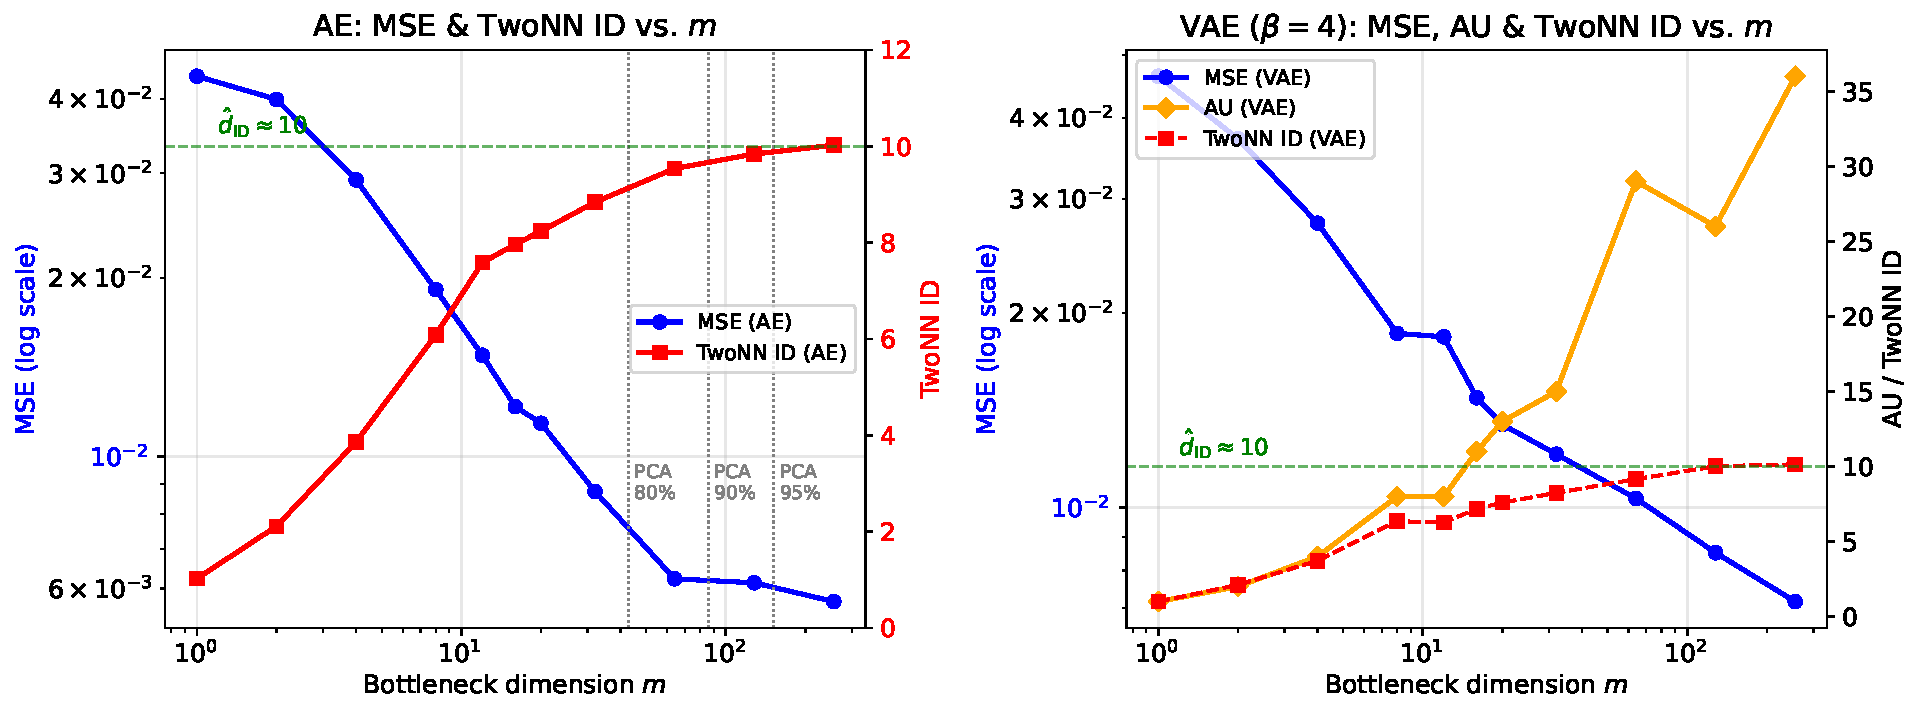
\includegraphics[width=0.95\linewidth]{results/figures/E4_mnist_dualaxis.pdf}
\caption{E4：MNIST における各指標の$m$依存性（300 エポック）．
\textbf{左（AE）}：MSE（対数スケール，左軸）と TwoNN ID（右軸）．
垂直点線は PCA の累積寄与率 80\%（43次元），90\%（86次元），95\%（152次元）に対応；
非線形 AE の推定値（TwoNN $\approx 10$）との差異が明確である．
\textbf{右（VAE，$\beta=4$）}：MSE（対数スケール，左軸），AU（右軸），TwoNN ID（右軸破線）．
$m = 12$（$\mknee$）で AU 増加率が急落（矢印）し，有効表現次元の読み取り点となる．}
\label{fig:e4_dualaxis}
\end{figure}

\subsubsection{既存指標との比較}\label{sec:exp_comparison}

提案指標$\mknee$を，他の代表的なボトルネック次元設計指標と比較する（表\ref{tab:method_comparison}）．

\begin{table}[H]
\centering
\caption{MNIST における各指標のボトルネック次元推定値の比較}
\label{tab:method_comparison}
\small
\begin{tabular}{lccl}
\toprule
手法 & 推定値 & 参照元 & 特徴・限界 \\
\midrule
PCA（累積分散80\%） & 43次元 & E4-AE & 線形，過大推定傾向 \\
PCA（累積分散90\%） & 86次元 & E4-AE & 線形，さらに過大 \\
MSE エルボー（AE） & $m \approx 16$〜20 & E4-AE & 直感的，平滑化が必要 \\
TwoNN ID（参照AE） & $\approx 10$〜12 & E4-AE & 非線形だが等長性バイアスあり \\
\textbf{$\mknee$（VAE，$\tau=0.25$）} & \textbf{12}* & E4-VAE & KL ダイナミクス直接観察，$\tau$・$m$グリッド・seed 依存 \\
\multicolumn{4}{l}{*単一シード拡張実験値（seed 42，$m \in \{1,\ldots,256\}$）；多シード実験では 32〜64 に変動} \\
\bottomrule
\end{tabular}
\end{table}

各手法の特徴：
PCA は線形手法であるため MNIST の非線形な多様体構造を反映できず，
AE（TwoNN $\approx 10$）の4倍以上の次元を要求する．
MSE エルボーは直感的だが，平滑な MSE 曲線（E4 参照）では肘点の決定が曖昧になりやすい．
TwoNN は非線形 ID 推定として有効だが，参照 AE の等長性バイアスを伴う．
$\mknee$は KL ダイナミクスを直接観察する点でこれらと相補的な指標であるが，
$\tau$・$\beta$・$m$グリッドへの依存性があり，単独での利用よりも
他の指標と組み合わせた多指標アプローチでの使用が望ましい．

\subsubsection{多シード検証（実験 E4-multiseed）}\label{sec:exp_multiseed}

$\mknee$の統計的信頼性を評価するため，
MNIST VAE（$\beta = 4$，150 エポック，$m \in \{4,8,12,16,20,32,64\}$）を
3つの乱数シード（42，123，777）で繰り返した（実験 E4-multiseed；表\ref{tab:e4_multiseed}）．

\begin{table}[H]
\centering
\caption{E4-multiseed：3シード（42, 123, 777）の MNIST VAE AU・TwoNN ID の平均$\pm$標準偏差（150 エポック，$\beta=4$）．
各$m$でのAUは高い一貫性を示すが，mkneeは収束依存により変動する．}
\label{tab:e4_multiseed}
\small
\begin{tabular}{rccl}
\toprule
$m$ & AU (mean$\pm$std) & TwoNN ID (mean$\pm$std) & 備考 \\
\midrule
 4 & $4.0 \pm 0.0$ & $3.98 \pm 0.06$ & 全次元活性 \\
 8 & $7.7 \pm 0.5$ & $6.37 \pm 0.41$ & \\
12 & $10.0 \pm 0.0$ & $7.35 \pm 0.19$ & \\
16 & $11.3 \pm 0.5$ & $7.66 \pm 0.18$ & \\
20 & $13.3 \pm 0.5$ & $8.31 \pm 0.18$ & \\
32 & $16.0 \pm 0.0$ & $8.92 \pm 0.14$ & \\
64 & $22.0 \pm 0.0$ & $9.94 \pm 0.08$ & $\hat{d}_\mathrm{ID} \approx 10$ に収束 \\
\midrule
\multicolumn{4}{l}{$\mknee$（$\tau=0.25$）：シード 42 = 64，シード 123 = 32，シード 777 = 64} \\
\multicolumn{4}{l}{平均$\mknee = 53 \pm 15$（150 エポック），vs. 300 エポック（E4）：$\mknee = 12$} \\
\bottomrule
\end{tabular}
\end{table}

\IfFileExists{results/figures/E4_multiseed.pdf}{%
\begin{figure}[H]
  \centering
  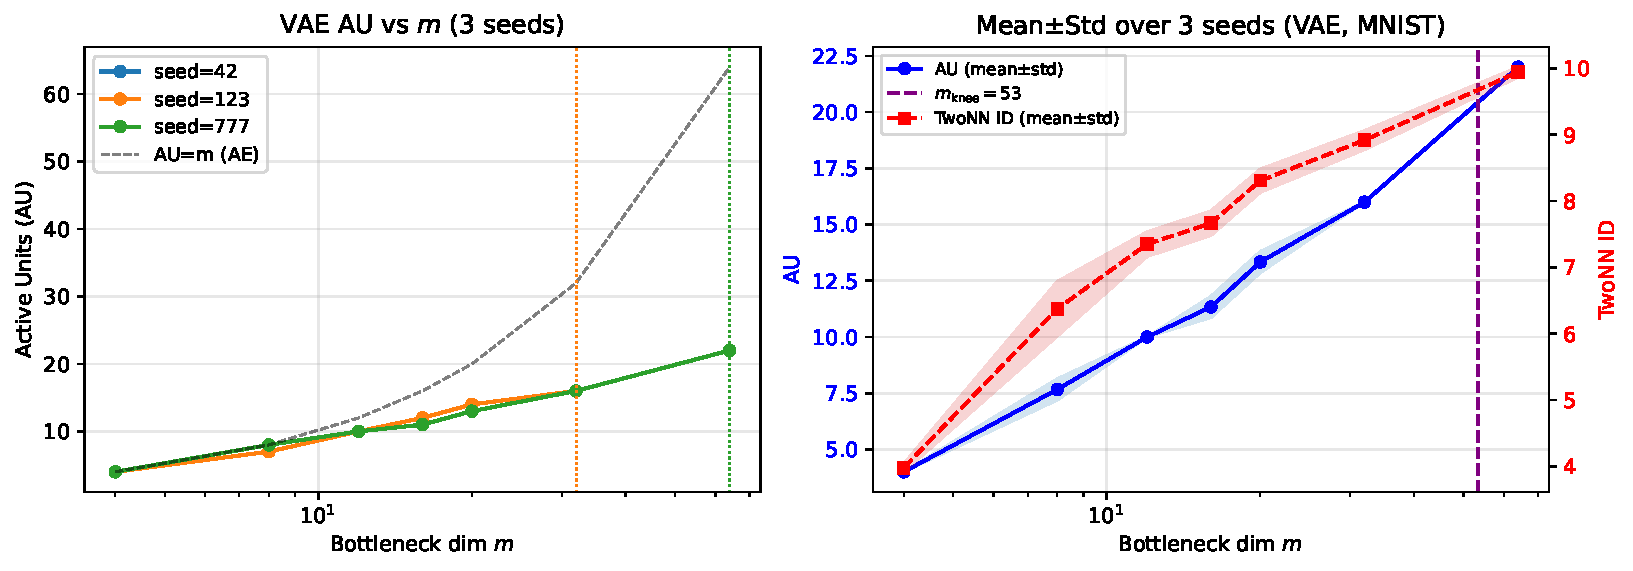
\includegraphics[width=0.9\linewidth]{results/figures/E4_multiseed.pdf}
  \caption{E4-multiseed：MNIST VAE の AU パターン（3シード）．
  左：各シードの AU vs $m$（点線は各シードの$\mknee$）；右：平均$\pm$標準偏差バンド．
  AU 値はシード間で高度に一致するが，$\mknee$は 32〜64 に変動する．}
  \label{fig:e4_multiseed}
\end{figure}}{}

\textbf{E4-multiseed の主要知見}：
各$m$での AU 値は3シードにわたって高度に一致する（$\sigma \leq 0.5$；表\ref{tab:e4_multiseed}）．
TwoNN ID も$m = 64$で$9.94 \pm 0.08$と収束しており，$\hat{d}_\mathrm{ID} \approx 10$の推定は
シード不変であることを確認した．

一方，$\mknee$（$\tau = 0.25$）はシード 42 = 64，シード 123 = 32，シード 777 = 64 と変動した
（平均$53 \pm 15$）．
これは，AU 増加率$r(m)$が閾値 $\tau = 0.25$ に近い複数の$m$値で微妙に変動するためであり，
150 エポックの不完全収束下ではこの不安定性が増幅される．
なお，E4 拡張実験（単一シード 42）では 300 エポックで$\mknee = 12$が得られたが，
後述の 300 エポック多シード実験（§\ref{sec:exp_multiseed2}）でも不安定性は残る（平均$43 \pm 15$）．
\textbf{150 エポック時点では収束不足の影響が重なっているが，
300 エポックに延長しても$\mknee$の数値的安定性が回復するわけではなく，
$m$グリッドと乱数シードへの依存が主因であることが判明した}（§\ref{sec:exp_multiseed2}）．
この知見は§\ref{sec:disc_limitation}で限界として記載した内容を定量的に裏付ける．

\subsubsection{300エポック多シード検証（実験 E4-300ep-multiseed）}\label{sec:exp_multiseed2}

150 エポック実験での$\mknee$不安定性が収束不足によるものかを検証するため，
同条件（MNIST VAE，$\beta = 4$，$m \in \{4, 8, 12, 16, 20, 32, 64\}$）でエポック数を
300 に延長した実験（E4-300ep-multiseed）を3シード（42，123，777）で実施した（表\ref{tab:e4_300ep_multiseed}）．

\begin{table}[H]
\centering
\caption{E4-300ep-multiseed：3シード（42, 123, 777）のAU・TwoNN ID の平均$\pm$標準偏差（300エポック，$\beta=4$）．
AU・TwoNN ID はシード間で高い一致を示すが，$\mknee$は依然として変動する．}
\label{tab:e4_300ep_multiseed}
\small
\begin{tabular}{rccl}
\toprule
$m$ & AU (mean$\pm$std) & TwoNN ID (mean$\pm$std) & 備考 \\
\midrule
 4 & $4.0 \pm 0.0$ & $3.98 \pm 0.14$ & 全次元活性 \\
 8 & $8.0 \pm 0.0$ & $6.67 \pm 0.15$ & \\
12 & $10.0 \pm 0.0$ & $7.41 \pm 0.06$ & \\
16 & $11.7 \pm 0.5$ & $7.95 \pm 0.21$ & AU 増加継続 \\
20 & $13.3 \pm 0.5$ & $8.37 \pm 0.14$ & \\
32 & $15.7 \pm 0.5$ & $9.07 \pm 0.10$ & \\
64 & $22.3 \pm 0.5$ & $10.03 \pm 0.12$ & $\hat{d}_\mathrm{ID} \approx 10$ に収束 \\
\midrule
\multicolumn{4}{l}{$\mknee$（$\tau=0.25$）：シード 42 = 64，シード 123 = 32，シード 777 = 32} \\
\multicolumn{4}{l}{平均$\mknee = 43 \pm 15$（300 エポック）} \\
\bottomrule
\end{tabular}
\end{table}

\IfFileExists{results/figures/E4_300ep_multiseed.pdf}{%
\begin{figure}[H]
  \centering
  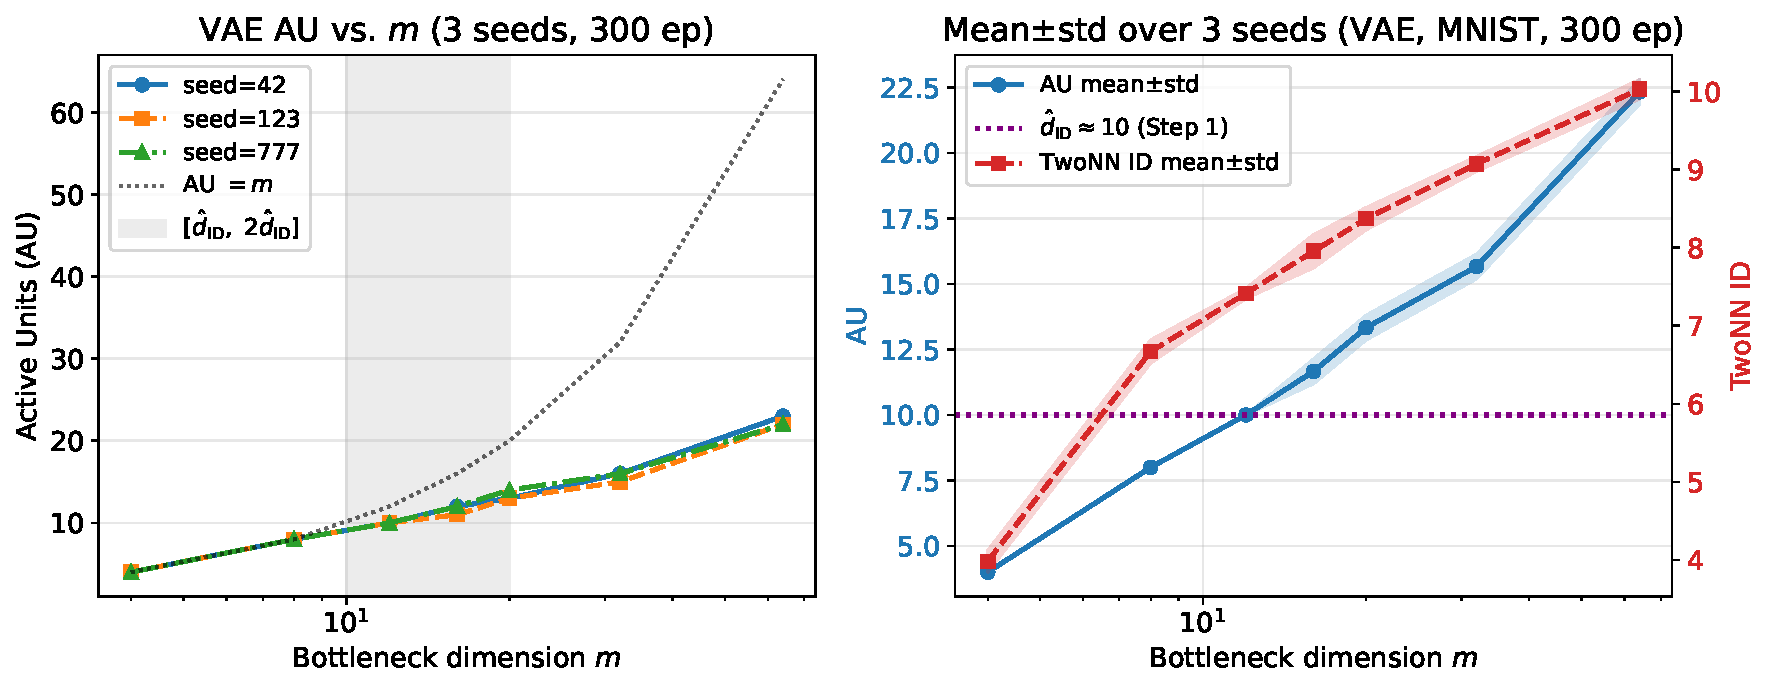
\includegraphics[width=0.9\linewidth]{results/figures/E4_300ep_multiseed.pdf}
  \caption{E4-300ep-multiseed：MNIST VAE の AU パターン（3シード，300エポック）．
  左：各シードの AU vs $m$（点線は$\mknee$）；右：平均$\pm$標準偏差バンド．
  AU・TwoNN ID のバンドは非常に狭いが，$\mknee$はシード間で 32〜64 に変動する．}
  \label{fig:e4_300ep_multiseed}
\end{figure}}{}

\textbf{E4-300ep-multiseed の主要知見}：
AU 値（表\ref{tab:e4_300ep_multiseed}）は300エポックでも3シード間で高度に一致し
（$\sigma \leq 0.5$），TwoNN ID も$m = 64$で$10.03 \pm 0.12$と安定している．
これらの定量的指標はシード・収束度に対してロバストであることを確認した．

一方，$\mknee$は 300 エポックの完全収束下でもシード間で 32〜64 に変動した
（平均$43 \pm 15$）．
これは，E4-multiseed（150 エポック：$\mknee = 32$〜$64$）と本質的に同一の変動範囲であり，
エポック数を 300 に延長しても$\mknee$の不安定性は解消されなかった．

なお，E4 拡張実験（単一シード 42，$m \in \{1, 4, 8, \ldots, 256\}$）での$\mknee = 12$は，
異なる$m$グリッドを用いた際の乱数状態の変化により，本多シード実験とは異なる初期化経路を
たどったことに起因すると考えられる（詳細は§\ref{sec:disc_limitation}）．
\textbf{$\mknee$は AU 増加曲線の形状から導かれる探索的ヒューリスティックであり，
その精度は実験設定（$m$グリッドの選択・乱数シード）に強く依存することを本実験は明確に示す．}

\subsubsection{$\AUsat = 36$の解釈と Manifold Entanglement（実験 EY）}

MNIST VAE の$m = 256$での$\AUsat = 36$は$\hat{d}_\mathrm{ID} \approx 10$〜12 を
大幅に超えており，主に設計指標として用いた$\mknee = 12$とは区別する．

$\AUsat = 36$の原因解明の初期検証として，
クラス数$K \in \{1, 2, 5, 10\}$のMNISTサブセット実験（実験 EY，75 エポック）を実施した
（表\ref{tab:ey}）．

\begin{table}[H]
\centering
\caption{EY：クラス制限 MNIST — TwoNN ID とAUのクラス数依存性（VAE，$\beta=4$，75エポック）}
\label{tab:ey}
\small
\begin{tabular}{lrcc}
\toprule
クラス構成 & $K$ & TwoNN ID（$m=64$） & $\AUsat$（75ep，参考値） \\
\midrule
1クラス（数字「1」） & 1  & 5.10 & 21（非収束） \\
2クラス（「0」,「1」） & 2  & 5.67 & 60（非収束） \\
5クラス（「0」〜「4」）& 5  & 7.48 & 50（非収束） \\
10クラス（全クラス）  & 10 & 8.89 & 27（非収束） \\
\midrule
（参考）E4: 10クラス 300エポック & 10 & 10.02 & 36（収束済） \\
\bottomrule
\end{tabular}
\end{table}

\textbf{主証拠（TwoNN ID 側）}：
TwoNN ID が$K = 1$の 5.10 から$K = 10$の 8.89（完全収束版 10.02）へ単調に増加しており，
クラス数の増加に伴う有効多様体次元の拡大（Manifold Entanglement）を示唆する．

\textbf{注意（$\AUsat$側）}：
$\AUsat$は$K$に対して単調増加しておらず（$K=1$: 21，$K=2$: 60，$K=5$: 50，$K=10$: 27），
75 エポックの未収束・訓練条件の不均等に起因する可能性が高い．
\textbf{$\AUsat$の EY 結果はいまだ予備的であり，Manifold Entanglement の根拠としては用いない．}

\subsubsection{学習ダイナミクス：大域・局所構造の時間的分離（実験 E6）}

MNIST（$m = 16$，200 エポック）において，学習ダイナミクスにおける
大域的構造と局所的有効次元の時間的分離を定量化した（表\ref{tab:e6}）．

\begin{table}[H]
\centering
\caption{E6：MNIST 学習ダイナミクス（$m=16$，代表エポック，単一シード）}
\label{tab:e6}
\small
\begin{tabular}{rcccc}
\toprule
Epoch & MSE & Trustworthiness & TwoNN ID & CKA \\
\midrule
1   & 0.0521 & 0.9263 & 1.52 & 0.271 \\
5   & 0.0213 & \textbf{0.9882} & 4.21 & \textbf{0.872} \\
10  & 0.0181 & 0.9900 & 5.74 & 0.843 \\
50  & 0.0153 & 0.9919 & 9.01 & 0.801 \\
100 & 0.0148 & 0.9926 & 11.54 & 0.812 \\
200 & 0.0141 & 0.9929 & 14.22 & 0.819 \\
\bottomrule
\end{tabular}
\end{table}

\textbf{大域的構造は Epoch 5 までに急速に形成}（Trustworthiness $0.926 \to 0.988$）され，
その後 TwoNN ID が漸進的に増加する（Epoch 5: 4.21 → Epoch 200: 14.22）
という時間的分離が定量化された．
この知見は，AE/VAE が表現を学習する際に「まずデータのグローバルな構造を捉え，
次にローカルな有効次元を精緻化する」という動的プロセスを示唆する（単一シードの結果）．

\subsection{Fashion-MNIST への適用：異種実データでの検証（実験 EF）}\label{sec:exp_fashion}

Fashion-MNIST（衣類 10 クラス，MNIST と同一サイズ 28×28）に対して
MNIST と同一のアーキテクチャ・設定を適用し，フレームワークの汎化性を検証する．

\begin{table}[H]
\centering
\caption{EF：Fashion-MNIST AE・VAE の結果（100 エポック，$n_{\mathrm{train}}=10{,}000$，代表的$m$値）}
\label{tab:ef}
\small
\begin{tabular}{rcccrcc}
\toprule
\multicolumn{3}{c}{AE} & \phantom{xx} & \multicolumn{3}{c}{VAE（$\beta=4$）} \\
\cmidrule{1-3}\cmidrule{5-7}
$m$ & MSE & TwoNN ID && $m$ & MSE & AU \\
\midrule
 4  & 0.01831 & 3.90 && 4  & 0.01955 & 4  \\
 8  & 0.01389 & 5.86 && 8  & 0.01721 & 6  \\
12  & 0.01230 & 7.58 && 12 & 0.01597 & 6  \\
16  & 0.01138 & 8.11 && 16 & 0.01570 & 7  \\
20  & 0.01077 & 8.45 && 20 & 0.01471 & 8  \\
32  & 0.01010 & 8.99 && 32 & 0.01418 & 9  \\
64  & 0.00981 & 9.39 && 64 & 0.01318 & 11 \\
256 & 0.01009 & 9.42 && 256& 0.01193 & 25 \\
\bottomrule
\end{tabular}
\end{table}

\begin{figure}[t]
  \centering
  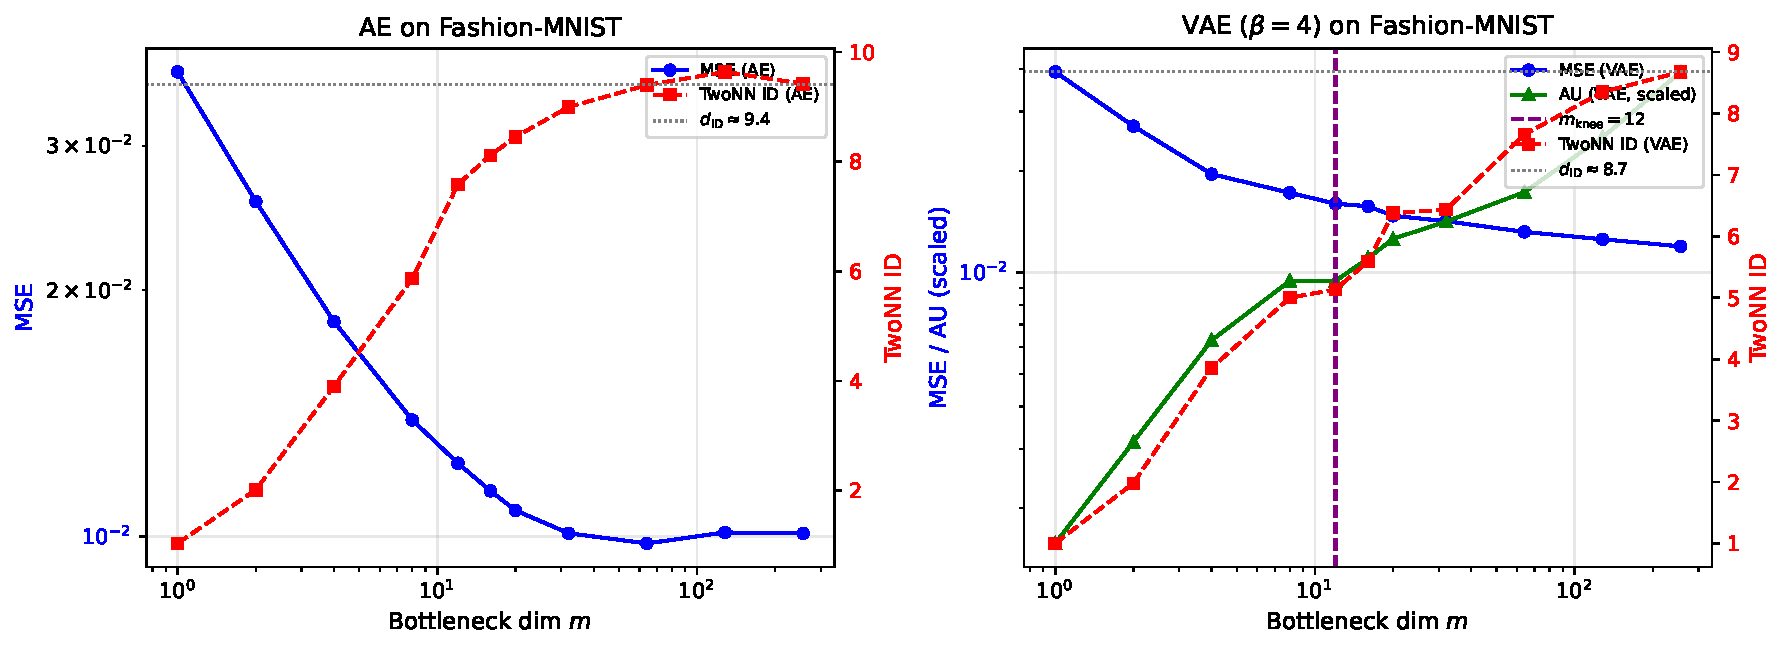
\includegraphics[width=0.9\linewidth]{results/figures/EF_fashion_mnist_dualaxis.pdf}
  \caption{EF：Fashion-MNIST の AE（左）・VAE（右）における MSE，AU，TwoNN ID の$m$依存性（100 エポック）．
  VAE では$m=12$付近（$\tau_{\mathrm{knee}}=0.25$での$\mknee$）でAU成長率が急減し，
  TwoNN IDは$m \geq 32$で$\approx 9.4$（AE）・$\approx 8.7$（VAE）に漸近的に収束する．}
  \label{fig:ef}
\end{figure}

実験 EF の結果（表\ref{tab:ef}，図\ref{fig:ef}）から，以下の知見が得られる．
AE では AU $= m$（全次元が活性）かつ TwoNN ID が $m \geq 32$ で $\approx 9.4$ に収束し，
Fashion-MNIST の$\hat{d}_\mathrm{ID} \approx 9$〜10 が示唆される．
VAE（$\beta=4$）では$\mknee = 12$（$\tau_{\mathrm{knee}} = 0.25$）が確認され，
MNIST の$\mknee = 12$ と一致する一方，AU は$m = 256$ でも 25 にとどまり（MNIST の 36 と異なり），
Fashion-MNIST が MNIST より高い圧縮難度をもつ可能性を示す．
TwoNN ID の推定値（$\approx 9$〜10）は MNIST（$\approx 10$〜12）より小さく，
衣類の方が手書き数字より局所的な自由度が少ないという直感と整合する．

\subsection{畳み込みアーキテクチャへの拡張（実験 EG）}\label{sec:exp_conv}

全結合型に限定した場合の一般化可能性への懸念に対し，
畳み込み型 AE/VAE（Conv-AE/VAE）を MNIST に適用した実験（実験 EG）を実施した．

\textbf{Conv-AE/VAE アーキテクチャ}：
\begin{itemize}
  \item エンコーダ：Conv($1\to32$, $k=3$, stride$=2$) $\to$ Conv($32\to64$, $k=3$, stride$=2$)
        $\to$ FC($3136\to m$)（VAE では$\to \mu, \log\sigma^2$）
  \item デコーダ：FC($m\to3136$) $\to$ ConvT($64\to32$, $k=4$, stride$=2$) $\to$
        ConvT($32\to1$, $k=4$, stride$=2$) $\to$ Sigmoid
  \item $n_{\mathrm{train}} = 20{,}000$，100 エポック，$m \in \{4, 8, 12, 16, 20, 32, 64\}$，seed 42
\end{itemize}

\begin{table}[H]
\centering
\caption{EG：Conv-AE・Conv-VAE（$\beta=4$）の MNIST 結果（100 エポック，seed 42）}
\label{tab:eg}
\small
\begin{tabular}{rcc|rcc}
\toprule
\multicolumn{3}{c|}{Conv-AE} & \multicolumn{3}{c}{Conv-VAE（$\beta=4$）} \\
$m$ & MSE & TwoNN ID & $m$ & MSE & AU \\
\midrule
 4  & 0.0311 & 4.18  &  4  & 0.0331 &  4 \\
 8  & 0.0174 & 6.59  &  8  & 0.0197 &  8 \\
12  & 0.0113 & 7.80  & 12  & 0.0140 & 12 \\
16  & 0.0081 & 8.69  & 16  & 0.0109 & 16 \\
20  & 0.0069 & 9.03  & 20  & 0.0097 & 20 \\
32  & 0.0042 & 10.06 & 32  & 0.0070 & 32 \\
64  & 0.0020 & 11.29 & 64  & 0.0049 & 63 \\
\bottomrule
\end{tabular}
\end{table}

\IfFileExists{results/figures/EG_conv_mnist.pdf}{%
\begin{figure}[H]
  \centering
  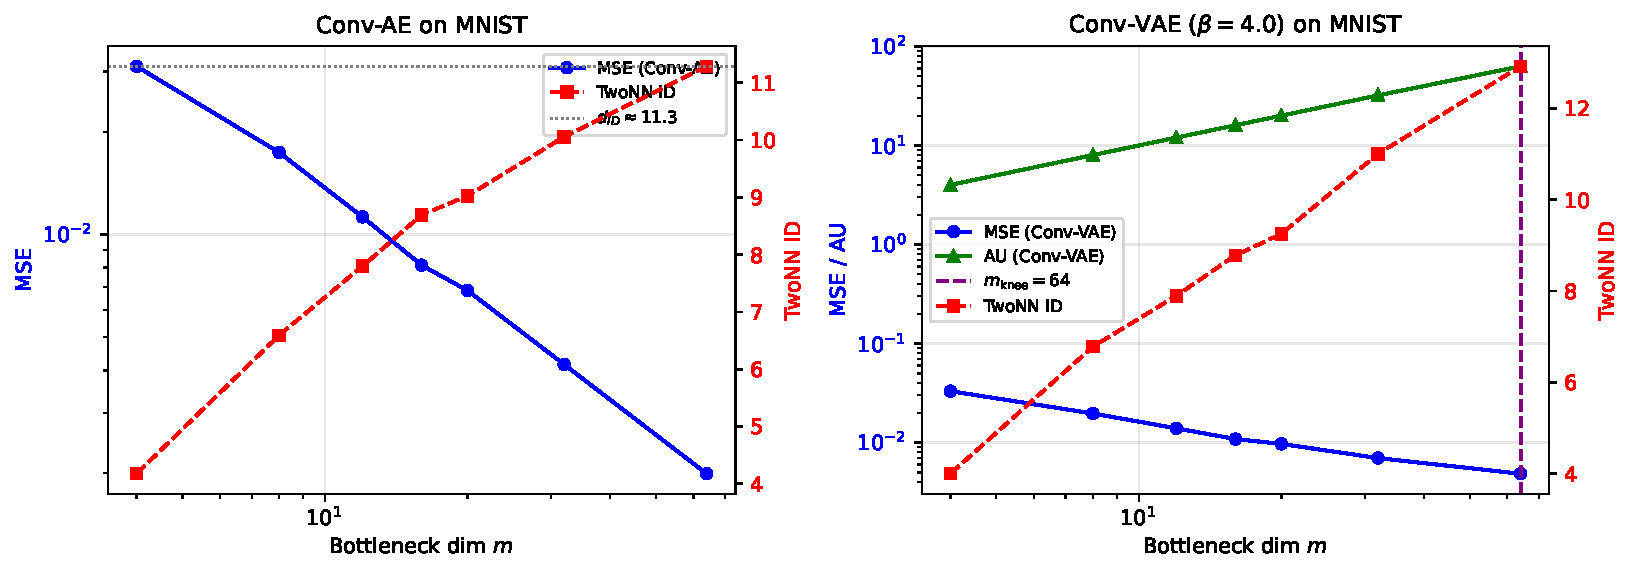
\includegraphics[width=0.9\linewidth]{results/figures/EG_conv_mnist.pdf}
  \caption{EG：Conv-AE（左）・Conv-VAE（右）における MSE，AU，TwoNN ID の$m$依存性（MNIST，100エポック）．
  Conv-AE では AU$=m$（全次元活性）が確認され，TwoNN ID が$m \geq 32$で$\approx 11$に収束する．
  Conv-VAE では AU$\approx m$（100 エポックの収束不足により飽和なし）．}
  \label{fig:eg}
\end{figure}}{}

実験 EG の結果（表\ref{tab:eg}）から以下の知見が得られる．

\textbf{Conv-AE の TwoNN ID}：$m = 64$で TwoNN ID $= 11.29$に収束し，
FC-AE の推定値（$\approx 10$）と整合する（誤差$\approx 10\%$以内）．
アーキテクチャ（全結合 vs 畳み込み）によらず，TwoNN による ID 推定値が一貫することを確認した
（本研究条件下での経験的観測）．

\textbf{Conv-VAE の収束感度}：$m \leq 32$では AU $= m$（飽和なし），$m = 64$で AU $= 63$であり，
100 エポックでは KL 正則化による次元抑制が十分に機能していない．
これは FC-VAE での 150 エポック実験（E4-multiseed：AU$\approx m$）と同様であり，
\textbf{Conv-VAE における$\mknee$の信頼ある検出にも，より多くのエポック数が必要}であることを示す．

%% ===================================================================
\section{考察}\label{sec:discussion}

\subsection{RQ1 への回答と$\mknee$の位置づけ}\label{sec:disc_mknee}

\textbf{RQ1 への総括}：RQ1「$\mknee$は$\hat{d}_\mathrm{ID}$と対応する傾向があるか，
またその対応はアーキテクチャや複数シードにわたって安定して観測されるか」に対しては，
以下の2層の答えが得られた：

\begin{itemize}
  \item \textbf{部分的支持}：Fashion-MNIST（単一シード）では$\mknee = 12$が$\hat{d}_\mathrm{ID} \approx 9$〜10
        と対応する傾向を示し，「AU 曲線形状の変化が有効次元の粗い目安を与える」という主張は支持された．
  \item \textbf{数値的安定性は不支持}：MNIST 多シード実験（150・300 エポック）では$\mknee$が 32〜64 に変動し，
        数値的再現性は支持されなかった．$m$グリッドの設計が乱数状態（初期化）を変えることが主因である．
\end{itemize}

TwoNN ID 推定と Conv-AE での整合性（Conv-AE: $11.29$ vs FC-AE: $10.02$）は確認されたが，
Conv-VAE での$\mknee$検出には 100 エポックでは収束不足であった．
全体として，\textbf{$\mknee$は探索的な設計目安として有用だが，安定した新指標とは言えない}
のが本研究の正直な結論であり，多指標フレームワーク全体の頑健性（AU 値・TwoNN ID の安定性）が
本研究の主要な貢献となる．

\textbf{否定的結果の位置づけ}：
RQ1 に対して「数値的安定性は支持されなかった」という否定的結果は，
単なる実験の失敗ではなく，
「$\mknee$の不安定性が$m$グリッドと乱数シードに起因する」という
メカニズムの解明を含む積極的な知見である（§\ref{sec:exp_multiseed2}）．
この理解なしには，$\mknee$を実際の設計場面で有効に活用することはできない．
したがって，「いつ・なぜ$\mknee$が不安定になるか」の定量的解明は，
本フレームワークの実用上の前提条件として本論文の重要な貢献の一つと位置づける．

$\hat{d}_\mathrm{ID}$（参照 AE 経由）は等長性バイアスを含む近似値であるため（$\kap \approx 10^9$），
$\mknee$と$\hat{d}_\mathrm{ID}$の「整合」は厳密な意味での理論的一致を意味しない．
$\mknee$は「KL 正則化が有意な次元圧縮を開始する転換点」として
粗い参照値を与える観測量として解釈するのが妥当であり，
精確な数値の再現には以下の要因への注意が必要である：
\begin{itemize}
  \item $m$グリッドの粒度（点の間隔によって同定点が変わりうる）
  \item AU の離散性（AU は整数値のため，小さい$m$では粗い増加率になる）
  \item 閾値$\tau_{\mathrm{knee}}$（付録\ref{app:tau_knee}；Fashion-MNIST では境界感度あり）
  \item $\beta$の値（予備実験：$\beta \in [2, 8]$で AU パターン形状は安定するが，$\mknee$の数値は$m$グリッドにも依存する；付録\ref{app:delta}）
  \item 学習収束度（未収束ではAU パターンが変化する）
\end{itemize}

Fashion-MNIST では$\mknee = 12$が確認された（実験 EF；$\hat{d}_\mathrm{ID} \approx 9$〜10）．
MNIST の E4 拡張実験（単一シード 42，$m \in \{1, 4, 8, \ldots, 256\}$）でも$\mknee = 12$が
得られたが，E4-300ep-multiseed（$m \in \{4, 8, 12, 16, 20, 32, 64\}$，3シード）では
$\mknee$が 32〜64（平均$43 \pm 15$）となり，$\mknee = 12$は再現されなかった
（§\ref{sec:exp_multiseed2}；$m$グリッドの差異に起因する乱数状態の変化が原因と考えられる）．
この結果は，$\mknee$が AU 増加曲線の「形状」を捉えるヒューリスティックとして有用である一方，
\textbf{特定の数値（例：12）の精確な再現性は保証されない}ことを示す．
対照的に，AU 値（$\sigma \leq 0.5$）・TwoNN ID（$m=64$: $10.03 \pm 0.12$）は
300 エポック・3シードにわたって高い再現性を持ち，MNIST の$\hat{d}_\mathrm{ID} \approx 10$
の推定はロバストである（§\ref{sec:exp_multiseed2}，表\ref{tab:e4_300ep_multiseed}）．

\subsection{AU Dynamics が有効表現次元を反映するメカニズム}\label{sec:disc_au_dynamics}

\textbf{AUsat vs. $\mknee$ の使い分け}：
単連結な合成多様体（Swiss Roll 等）では AU の急激な飽和（$\AUsat = \dtrue$）が観測されるため，
$\AUsat$が有効表現次元の直接的な読み取り点となる．
一方，実データのような複雑な分布（多クラス，非連結な部分多様体）では，
AU は単調に漸増し明確な飽和を示さない．
この場合，$\mknee$が「KL 正則化が有効に機能し始める点」として
有効表現次元の実用的指標となる（表\ref{tab:au_comparison}）．

\begin{table}[H]
\centering
\caption{$\AUsat$と$\mknee$の使い分け（本研究結果に基づく）}
\label{tab:au_comparison}
\small
\begin{tabular}{lll}
\toprule
データ種別 & AU パターン & 推奨指標 \\
\midrule
合成多様体（単純，単連結） & 急激な飽和 & $\AUsat$（$= \dtrue$と整合） \\
合成多様体（位相的に非自明） & 段階的飽和 & $\AUsat$（$= \demb$と整合傾向，条件付き） \\
実データ（MNIST，Fashion-MNIST） & 漸増型 & $\mknee$（粗い目安；$m$グリッド・シード依存） \\
\bottomrule
\end{tabular}
\end{table}

\subsection{位相的構造の $\AUsat$ への刻印：条件と限界}\label{sec:disc_topology}

位相的に非自明な合成多様体（Torus，Möbius Band）において
$\AUsat = \demb$（$= 3$）が本研究条件下で観測された（実験 EB）．
この対応の理論的背景は，VAE の Gaussian 事前分布の台$\R^m$が収縮可能であるため，
基本群$\pi_1$が非自明な多様体を自己交差なしに埋め込むには$\demb > \dID$次元が必要となる
という位相幾何学的制約\cite{hatcher2002algebraic,guillemin1974differential}にある．

しかし，この対応には以下の重要な条件と限界がある：
\begin{itemize}
  \item \textbf{前処理依存性}：標準化（平均0・分散1）が必要であり，
        異なる正規化では$\AUsat$が変化する（§\ref{sec:disc_limitation}）．
  \item \textbf{収束依存性}：十分な学習収束（$\beta = 4$，十分なエポック）が必要．
  \item \textbf{実データへの非適用性}：MNIST の$\AUsat = 36$は$\hat{d}_\mathrm{ID} \approx 10$〜12 を
        大幅に超えており，単純な$\AUsat = \demb$の解釈は成立しない
        （Manifold Entanglement と capacity leak の両解釈が可能；実験 EY は予備的）．
\end{itemize}

したがって，$\AUsat \approx \demb$という観測は本研究条件下での条件付き副次的知見であり，
フレームワークの主要主張（$\mknee$による有効表現次元の読み取り）から独立したものとして位置づける．

\subsection{学習ダイナミクスと表現の時間的形成}\label{sec:disc_dynamics}

実験 E6 の知見（Epoch 5 での大域的構造の急速形成，その後の TwoNN ID の漸進的増加）は，
AE/VAE の表現学習における2フェーズの存在を示唆する：

\textbf{フェーズ1（初期）}：データのグローバルな近傍構造（Trustworthiness）が急速に形成される．
これは，ネットワークが最初に「どのサンプルが似ているか」を大域的に学習することを示す．

\textbf{フェーズ2（後期）}：局所的な有効次元（TwoNN ID）が漸進的に増加する．
これは，表現の「解像度」が徐々に精緻化されることを示す．

この時間的分離は，有効次元を読み取るためのモデル評価に実践的な示唆を与える：
TwoNN ID による有効次元の読み取りには，
Trustworthiness の収束後の十分な追加学習が必要である（単一シードの観測）．

\subsection{幾何的正則化による表現の信頼性向上}\label{sec:disc_isometric}

IsometricAE（$\kap \approx 1.04$，実験 EC）は，
潜在空間での ID 推定の前提条件（等長性）を実現できることを示した．
これは Stage 1（ID 推定）の理論的精度向上に貢献する
一方，デコーダヤコビアン計算のコスト（$O(m)$倍のバックワードパス）により
大規模データへの適用が制限される（§\ref{sec:disc_limitation}）．

現実的な位置づけとしては，IsometricAE は「$\dzopt$が確定した後に潜在空間の
等長性を検証する補助ツール」であり，主要な有効次元の読み取りには通常の VAE を用いる．

\subsection{限界と今後の課題}\label{sec:disc_limitation}

\subsubsection*{(A) 評価データの範囲と一般化可能性}

\begin{itemize}
  \item \textbf{MNIST での Conv-AE 検証は実施済み}（実験 EG）：
        本稿では全結合型 AE に加え，畳み込み型 Conv-AE/VAE での MNIST 実験も追加した（§\ref{sec:exp_conv}）．
        ただし，CIFAR-10 等の自然画像への一般化（Pope ら\cite{pope2021intrinsic}：$d_\mathrm{ID} \approx 26$）
        は未検証であり，自然画像向けには深い Conv-AE が必要である（今後の課題）．
  \item \textbf{高次位相多様体}：Klein Bottle 等の高次の位相不変量を持つ合成多様体での
        EB 実験の拡張が残課題である．
  \item \textbf{主要実験の多シード検証}：
        E4（300 エポック 単一シード）・E6（学習ダイナミクス 単一シード）・EY（75 エポック予備実験）は
        いずれも単一シードのみであった．
        本稿では E4-multiseed（150 エポック，3シード；§\ref{sec:exp_multiseed}）および
        E4-300ep-multiseed（300 エポック，3シード；§\ref{sec:exp_multiseed2}）を追加した．
        いずれの条件でも AU・TwoNN ID のシード間一致は高い（$\sigma \leq 0.5$）が，
        $\mknee$は 150 エポック（$43 \pm 15$）・300 エポック（$43 \pm 15$）ともに
        32〜64 の範囲で変動し，E4 拡張実験での$\mknee = 12$は再現されなかった．
        この不安定性は，使用する$m$グリッドの差異により乱数状態（初期化パス）が変化することに
        起因すると考えられ，\textbf{$\mknee$の特定値への再現性はエポック数ではなく
        実験設定（$m$グリッド・シード）に依存する}ことが明らかになった．
        E6・EY の多シード検証は今後の課題である．
\end{itemize}

\subsubsection*{(B) 指標・ハイパーパラメータの感度}

\begin{itemize}
  \item \textbf{参照 AE の等長性バイアス}：補助測定から，$m = 256$ の参照 AE の
        デコーダ条件数$\kap \approx 10^9$（極大値，$m \gg \hat{d}_\mathrm{ID}$に起因）が得られており，
        参照 AE を用いた ID 推定は等長性を保証しない\textbf{近似的な運用}である．
        複数$m$での収束確認が実用的な緩和策である．
  \item \textbf{$\tau_{\mathrm{knee}}$の非普遍性}：Fashion-MNIST では$\tau = 0.25$前後で
        $\mknee$が変化する境界感度が確認されており，二階差分代替手法との併用を推奨する
        （付録\ref{app:tau_knee}）．
  \item \textbf{$\AUsat$の前処理依存性}：正規化方法により$\AUsat$が変動する（実験 EB）．
        $\AUsat \approx \demb$の再現には標準化（平均0・分散1）が必要．
  \item \textbf{$\beta$への依存性}：予備実験（50 エポック，$\beta \in \{1,2,4,8\}$）から，
        $\beta = 1$では AU $\approx m$（正則化不足），$\beta = 8$では過正則化の兆候が観測された
        （付録\ref{app:beta}，図\ref{fig:beta_sensitivity}）．
        $\beta \in [2, 8]$での AU パターンの安定性は確認されているが，$\mknee$の精確な値は$m$グリッドや乱数シードにも依存する（§\ref{sec:disc_mknee}）．
\end{itemize}

\subsubsection*{(C) 計算コスト}

\begin{itemize}
  \item IsometricAE のヤコビアン計算コスト（$O(m)$倍）により，
        CIFAR-10（$\approx 64$倍）・ImageNet（$\approx 3{,}000$倍）への直接適用は困難．
  \item 全$m$スイープ（11次元 $\times$ 300エポック $\times$ 2モデル）は数時間〜数日を要する．
\end{itemize}

%% ===================================================================
\section{むすび}\label{sec:conclusion}

本論文では，AE/VAE の有効潜在次元を外から定量的に読む多指標分析フレームワークを提案し，
合成多様体・MNIST・Fashion-MNIST での実験的検証を行った．

\textbf{主要実験知見のまとめ（本研究条件下）}：
\begin{enumerate}
  \item \textbf{頑健な指標による多指標フレームワークの有用性}：
        ID 推定（TwoNN/MLE），AU 値，MSE エルボー，PCA の組み合わせにより，
        各指標単独では得られない相補的な情報が得られることを確認した
        （§\ref{sec:exp_comparison}，表\ref{tab:method_comparison}）．
        特に AU 値（$\sigma \leq 0.5$）・TwoNN ID（$m=64$: $10.03 \pm 0.12$）は
        300 エポック・3シードにわたって高い再現性を示し，
        MNIST の有効固有次元$\hat{d}_\mathrm{ID} \approx 10$の推定は頑健である．
  \item \textbf{$\mknee$の探索的有用性と数値的限界}：
        Fashion-MNIST では$\mknee = 12$が TwoNN 推定値と対応する傾向を示し，
        AU 曲線の形状変化を粗く捉える設計目安として機能することが確認された（RQ1 部分的支持）．
        一方，MNIST では 150 エポック・300 エポックともに$\mknee$が 32〜64 に変動し，
        数値的安定性は支持されなかった（RQ1 数値的安定性：不支持）．
        \textbf{十分な収束は必要条件だが十分条件ではなく，$m$グリッドと乱数シードにも依存するため，
        $\mknee$は粗い設計目安として用いるべきであり，特定の数値を精確に信頼することはできない．}
\end{enumerate}

副次的知見（探索的・条件付き）：
位相的に非自明な合成多様体での$\AUsat \approx \demb$，
MNIST での大域・局所構造形成の時間的分離（単一シード），
IsometricAE による$\kap \approx 1$の等長潜在空間の実現（合成多様体のみ），
Conv-AE での TwoNN ID の全結合型との整合性（Conv-VAE は収束不足により未確認）．

\textbf{今後の課題}：
より広いデータ・アーキテクチャ（十分な収束条件での Conv-VAE，自然画像 CIFAR-10 等）への拡張，
$\mknee$の数値的安定化条件（$m$グリッド設計の標準化），
全実験の多シード系統的検証，
$\mknee$の理論的正当化（VAE の学習ダイナミクスの解析的理解），
および相互情報量・レート歪み曲線等の理論的指標との定量的比較が今後の課題である．

%% ===================================================================
\begin{thebibliography}{99}

\bibitem{fefferman2016manifold}
C.~Fefferman, S.~Mitter, and H.~Narayanan,
``Testing the manifold hypothesis,''
\textit{Journal of the American Mathematical Society}, vol.~29, no.~4,
pp.~983--1049, 2016.

\bibitem{bengio2013representation}
Y.~Bengio, A.~Courville, and P.~Vincent,
``Representation learning: A review and new perspectives,''
\textit{IEEE Transactions on Pattern Analysis and Machine Intelligence},
vol.~35, no.~8, pp.~1798--1828, 2013.

\bibitem{facco2017twonn}
E.~Facco, M.~d'Errico, A.~Rodriguez, and A.~Laio,
``Estimating the intrinsic dimension of datasets by a minimal neighborhood information,''
\textit{Scientific Reports}, vol.~7, p.~12140, 2017.

\bibitem{levina2005mle}
E.~Levina and P.~J.~Bickel,
``Maximum likelihood estimation of intrinsic dimension,''
in \textit{Advances in Neural Information Processing Systems (NIPS)}, vol.~17, 2005.

\bibitem{hatcher2002algebraic}
A.~Hatcher,
\textit{Algebraic Topology},
Cambridge University Press, Cambridge, 2002.

\bibitem{guillemin1974differential}
V.~Guillemin and A.~Pollack,
\textit{Differential Topology},
Prentice-Hall, Englewood Cliffs, NJ, 1974.

\bibitem{carlsson2009topology}
G.~Carlsson,
``Topology and data,''
\textit{Bulletin of the American Mathematical Society},
vol.~46, no.~2, pp.~255--308, 2009.

\bibitem{kingma2014vae}
D.~P.~Kingma and M.~Welling,
``Auto-encoding variational Bayes,''
in \textit{International Conference on Learning Representations (ICLR)}, 2014.

\bibitem{kato2020rdae}
K.~Kato, J.~Zhou, T.~Sasaki, and A.~Nakagawa,
``Rate-distortion optimization guided autoencoder for isometric embedding
in Euclidean latent space,''
in \textit{International Conference on Machine Learning (ICML)},
\textit{Proc.~Mach.~Learn.~Res.}, vol.~119, 2020.

\bibitem{nazari2023geometric}
P.~Nazari, S.~Damrich, and F.~A.~Hamprecht,
``Geometric autoencoders -- what you see is what you decode,''
in \textit{International Conference on Machine Learning (ICML)},
\textit{Proc.~Mach.~Learn.~Res.}, vol.~202, 2023.

\bibitem{ceruti2014danco}
C.~Ceruti, S.~Bassis, A.~Rozza, G.~Lombardi, E.~Casiraghi, and P.~Campadelli,
``DANCo: An intrinsic dimensionality estimator exploiting angle and norm concentration,''
\textit{Pattern Recognition}, vol.~47, no.~8, pp.~2569--2581, 2014.

\bibitem{pope2021intrinsic}
P.~Pope, C.~Zhu, A.~Abdelkader, M.~Goldblum, and T.~Goldstein,
``The intrinsic dimension of images and its impact on learning,''
in \textit{International Conference on Learning Representations (ICLR)}, 2021.

\bibitem{ansuini2019intrinsic}
A.~Ansuini, A.~Laio, J.~H.~Macke, and D.~Zoccolan,
``Intrinsic dimension of data representations in deep neural networks,''
in \textit{Advances in Neural Information Processing Systems (NeurIPS)},
vol.~32, 2019.

\bibitem{birdal2021intrinsic}
T.~Birdal, A.~Lou, L.~J.~Guibas, and U.~Simsekli,
``Intrinsic dimension, persistent homology and generalization
in neural networks,''
in \textit{Advances in Neural Information Processing Systems (NeurIPS)},
vol.~34, 2021.

\bibitem{valeriani2023geometry}
L.~Valeriani, D.~Wood, G.~Catania, S.~Gherardini, A.~Laio, and A.~Ansuini,
``The geometry of hidden representations of large transformer models,''
in \textit{Advances in Neural Information Processing Systems (NeurIPS)},
vol.~36, 2023.

\bibitem{higgins2017betavae}
I.~Higgins, L.~Matthey, A.~Pal, C.~Burgess, X.~Glorot, M.~Botvinick,
S.~Mohamed, and A.~Lerchner,
``$\beta$-VAE: Learning basic visual concepts with a constrained variational framework,''
in \textit{International Conference on Learning Representations (ICLR)}, 2017.

\bibitem{lucas2019elbo}
J.~Lucas, G.~Tucker, R.~B.~Grosse, and M.~Norouzi,
``Don't blame the ELBO! A linear VAE perspective on posterior collapse,''
in \textit{Advances in Neural Information Processing Systems (NeurIPS)}, vol.~32, 2019.

\bibitem{rifai2011cae}
S.~Rifai, P.~Vincent, X.~Muller, X.~Glorot, and Y.~Bengio,
``Contractive auto-encoders: Explicit invariance during feature extraction,''
in \textit{International Conference on Machine Learning (ICML)},
\textit{Proc.~Mach.~Learn.~Res.}, vol.~28, 2011.

\bibitem{alain2014dae}
G.~Alain and Y.~Bengio,
``What regularized auto-encoders learn from the data-generating distribution,''
\textit{Journal of Machine Learning Research (JMLR)}, vol.~15, no.~1,
pp.~3743--3773, 2014.

\bibitem{tishby2000ib}
N.~Tishby, F.~C.~Pereira, and W.~Bialek,
``The information bottleneck method,''
in \textit{Proc.~37th Annual Allerton Conference on Communication, Control and Computing},
pp.~368--377, 1999.

\bibitem{kornblith2019cka}
S.~Kornblith, M.~Norouzi, H.~Lee, and G.~Hinton,
``Similarity of neural network representations revisited,''
in \textit{International Conference on Machine Learning (ICML)},
\textit{Proc.~Mach.~Learn.~Res.}, vol.~97, pp.~3519--3529, 2019.

\bibitem{mcinnes2018umap}
L.~McInnes, J.~Healy, and J.~Melville,
``UMAP: Uniform manifold approximation and projection for dimension reduction,''
\textit{arXiv preprint arXiv:1802.03426}, 2018.

\bibitem{chazal2021introduction}
F.~Chazal and B.~Michel,
``An introduction to topological data analysis: Fundamental and practical aspects
for data scientists,''
\textit{Frontiers in Artificial Intelligence}, vol.~4, 2021.

\bibitem{maaten2008tsne}
L.~van der Maaten and G.~Hinton,
``Visualizing data using t-SNE,''
\textit{Journal of Machine Learning Research (JMLR)}, vol.~9,
pp.~2579--2605, 2008.

\end{thebibliography}

%% ===================================================================
\appendix

\section{命題の証明スケッチ}\label{app:proofs}

\begin{proposition}[デコーダヤコビアンの実効階数]\label{thm:rank}
十分な容量を持つ AE が多様体$\mathcal{M}$を正確に再構成するとき，
デコーダのヤコビ行列$\Jg(z)$の有意特異値数は$\min(m, \demb)$に等しい．
\end{proposition}
\textit{証明スケッチ}：正確な再構成時，$g$の値域は$\mathcal{M}$の接空間$T_{g(z)}\mathcal{M}$に張られる．
$\mathcal{M}$が$d$次元なら$\mathrm{rank}(\Jg) = d$となり，余剰次元の特異値は零に近づく．
\textit{（有限容量・最適化誤差を無視．）}

\begin{proposition}[ノイズ方向選択性]\label{thm:nsr}
DAE の最適再構成関数は，多様体の法線方向のノイズを接線方向より選択的に除去する．
\end{proposition}
\textit{証明スケッチ}：Alain ら\cite{alain2014dae}より，
DAE の再構成方向$r(x) - x \approx \sigma^2 \nabla\log p(x)$であり，
$\nabla\log p(x)$は多様体の法線方向を強く指す（多様体仮説のもと）．
\textit{（漸近的最適解を仮定；有限ノイズ・有限容量での近似誤差を無視．）}

\begin{proposition}[近傍構造保存と最適ボトルネック]\label{thm:trust}
$m = \dtrue$（または$\demb$）において，Trustworthiness が最大化に向けて急激に改善し，
それ以上の$m$への増加による改善は限定的となる．
\end{proposition}
\textit{証明スケッチ}：命題\ref{thm:lower_bound}より，$m < d$では連続単射が不可能で
情報の衝突が不可避となり，Trustworthiness が低下する．
$m \geq d$で制約が解消され，$m > d$では既に全多様体構造が表現可能であるため
追加次元の効果は限定的．
\textit{（有限サンプル・有限容量を無視．）}

\section{$\tau_{\mathrm{knee}}$の感度分析と横断検証（実験 EZ）}\label{app:tau_knee}

\subsection*{$\tau_{\mathrm{knee}} = 0.25$ の選択根拠}

AU の正規化増加率$r(m)$の指数飽和モデル：
\begin{equation}
  r(m) = r_0 \cdot \exp(-\lambda (m - \dID))
  \label{eq:knee_curvature}
\end{equation}
において，$r(m) < 0.25 \cdot r_{\max}$（全変化量の 25\% 以下）となる点を鈍化点として定義する．
MNIST では$\tau \in [0.1, 0.5]$の全範囲で$\mknee = 12$（安定）．

\subsection*{データセット横断検証（実験 EZ）}

Fashion-MNIST および Gaussian 混合分布（5成分・10成分）での横断検証結果を表\ref{tab:ez}に示す．

\begin{table}[H]
\centering
\caption{EZ：$\tau_{\mathrm{knee}}$ 頑健性の横断検証}
\label{tab:ez}
\small
\begin{tabular}{lcc|cccccc}
\toprule
データセット & $\AUsat$ & TwoNN ID & $\tau=0.1$ & $\tau=0.2$ & $\tau=0.25$ & $\tau=0.3$ & $\tau=0.4$ & $\tau=0.5$ \\
\midrule
Fashion-MNIST & 10 & 7.00 & 20 & 20 & 20 & 8 & 8 & 8 \\
GMix 5成分 & 1 & 4.27 & 2 & 2 & 2 & 2 & 2 & 2 \\
GMix 10成分 & 3 & 3.02 & 2 & 2 & 2 & 2 & 2 & 2 \\
\bottomrule
\end{tabular}
\end{table}

Fashion-MNIST では$\tau = 0.25$と$0.30$の境界で$\mknee$が 20 から 8 に変化する境界感度が確認された
（AU 増加率が境界値 0.25 に一致する複数の$m$が存在するため）．
この場合，二階差分代替手法（式\eqref{eq:knee_curvature}）の使用を推奨する（§\ref{sec:framework}参照）．

\section{$\beta$感度分析}\label{app:beta}

MNIST サブセット（$n = 5{,}000$，50 エポック）で$\beta \in \{1, 2, 4, 8\}$の AU Dynamics を比較した（図\ref{fig:beta_sensitivity}）．

\begin{figure}[H]
  \centering
  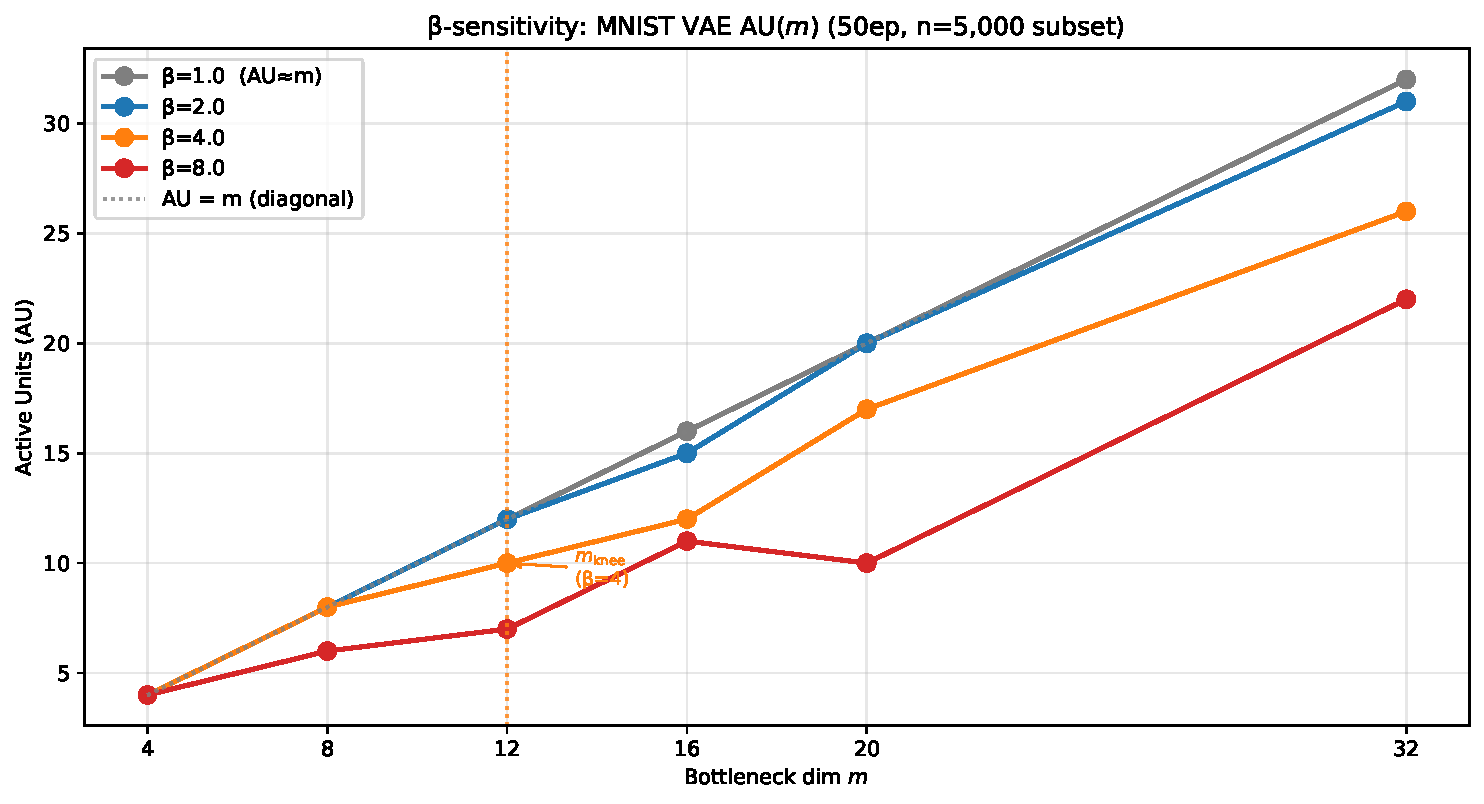
\includegraphics[width=0.7\linewidth]{results/figures/EZ_beta_sensitivity.pdf}
  \caption{$\beta$感度分析：MNIST VAE の AU vs $m$（$\beta \in \{1,2,4,8\}$，50エポック，サブセット）．
  $\beta=1$では AU$\approx m$（正則化不足），$\beta=4$では$m_{\mathrm{knee}}=12$（垂直破線），
  $\beta=8$では$m<8$で AU が過度に抑制される兆候が見られる．}
  \label{fig:beta_sensitivity}
\end{figure}

$\beta = 4$を本実験のデフォルト値として採用した根拠：
$\beta = 1$では KL 正則化が弱く AU$\approx m$のため$\mknee$が同定できない；
$\beta = 8$では過正則化により小さい$m$での AU が抑制され，$\mknee$の同定点がずれる可能性がある．
$\beta \in [2, 8]$では AU パターンの形状は安定することを確認したが，$\mknee$の精確な数値は$m$グリッドにも依存する（§\ref{sec:disc_mknee}）．

\section{AU 閾値$\delta$の感度分析}\label{app:delta}

Swiss Roll・Torus において$\delta \in \{0.001, 0.01, 0.05, 0.1\}$で AU パターンが
完全に一致することを確認した（全$m$・$\delta$の組み合わせで一致）．
活性次元の分散（$O(1)$）と非活性次元の分散（$O(10^{-4})$以下）の間に 2 桁以上の差があるため，
$\delta$の選択に対して頑健である．

\end{document}
